\documentclass[11pt,a4paper]{article}
\usepackage{fontspec}
\setmainfont{Latin Modern Roman}
\setsansfont{Latin Modern Sans}
\setmonofont{Latin Modern Mono}
\usepackage{unicode-math}
\setmathfont{Latin Modern Math}
\usepackage[a4paper,margin=2.5cm]{geometry}
\usepackage{graphicx,booktabs,longtable,array,calc,float}
\usepackage[font=small,labelfont=bf]{caption}
\usepackage[round,authoryear]{natbib}
\usepackage{xcolor}
\usepackage[colorlinks=true,linkcolor=black,citecolor=black,urlcolor=blue!50!black]{hyperref}
\usepackage{fancyhdr}
\usepackage{tikz}
\usetikzlibrary{positioning,arrows.meta}
\usepackage{microtype}
\setlength{\parskip}{0.5em}\setlength{\parindent}{0pt}
\renewcommand{\arraystretch}{1.2}
\providecommand{\tightlist}{\setlength{\itemsep}{0pt}\setlength{\parskip}{0pt}}
\pagestyle{fancy}\fancyhf{}
\fancyhead[L]{\small Bubble Size Measurement in a Novel Flotation Technology}
\fancyhead[R]{\small T.~Trieu}
\fancyfoot[C]{\small\thepage}
\renewcommand{\headrulewidth}{0.4pt}
\begin{document}
\begin{titlepage}
\centering

\includegraphics[width=3cm]{crest.png}\par\vspace{1.2cm}
{\large UNSW Sydney\par School of Minerals and Energy Resources Engineering\par}
\vspace{2.5cm}
{\LARGE\bfseries Bubble Size Measurement in a\\[2pt] Novel Flotation Technology\par}
\vspace{0.8cm}
{\large Deep-learning measurement of bubble size and Sauter mean diameter\\ from pulp and froth video\par}
\vspace{2.5cm}
{\large Taste of Research Technical Report\par}
\vspace{1.8cm}
{\large Tristan (Quoc Anh) Trieu\par}
{\normalsize zID: z5793457\par}
\vspace{0.8cm}
{\normalsize Supervisor: Prof Seher Ata\par}
\vfill
{\normalsize Faculty of Engineering Taste of Research Scholarship, Term 2--Term 3\par November 2026\par}
\end{titlepage}
\begin{abstract}
\noindentBubble size controls how much mineral a flotation cell recovers, and it is
summarised by the Sauter mean diameter (D32). In practice D32 is still
measured from video largely by hand, which is slow and subjective. This
project built BubbleMetrix, a desktop tool that measures bubble size and
D32 automatically from flotation video, for both the pulp and the froth
zone.

For the pulp, a Mask R-CNN instance segmentation model was trained on
hand-labelled probe footage. Tested on operating conditions it had never
seen, it measured D32 within 1.5\% of careful hand measurement on average
(ratio 0.99 ± 0.03 over 8 conditions), as consistent as a person repeating
their own measurement. For the froth, Cellpose, a general-purpose
segmentation model, was used without any froth-specific training. It found
86\% of hand-outlined bubbles and gave a steady D32 of 2.16 mm, in under a
minute per frame.

BubbleMetrix needs no machine-learning knowledge to use: it measures a
whole video in one step, reports D32 with a 95\% confidence interval, stops
once D32 is known to ±5\%, and can be fine-tuned on new footage when a
quick check shows it is needed.

\end{abstract}
\setcounter{tocdepth}{1}\tableofcontents
\newpage
\hypertarget{introduction}{%
\section{Introduction}\label{introduction}}

Flotation separates valuable minerals from waste rock by attaching the
mineral particles to rising air bubbles. Smaller bubbles carry more
surface area per unit of gas, so bubble size directly sets how much
mineral a cell can capture.

Engineers summarise a bubble population with the Sauter mean diameter,
the diameter of a bubble with the same volume-to-surface ratio as the
whole population:

\[D_{32} = \frac{\sum_i d_i^3}{\sum_i d_i^2}\]

The project's novel flotation cell is filmed by a probe in the pulp and
by a camera on the froth column. Measuring bubbles from that video by
hand is slow and subjective. Most pulp bubbles are out of focus or
overlapping, and only sharp ones can be sized accurately.

The project inherited BubMask-Fiji, a Mask R-CNN tool built by a
previous student. It had never been tested against independent hand
counts on this footage (Section~4).

\textbf{Aims}

\begin{enumerate}
\def\labelenumi{\arabic{enumi}.}
\tightlist
\item
  Automate bubble sizing from pulp-zone probe video.
\item
  Match hand measurement for D32, tested on operating conditions the
  model has never seen.
\item
  Extend the method to the froth zone.
\item
  Deliver a tool researchers can use without any machine-learning
  knowledge.
\end{enumerate}

\hypertarget{background}{%
\section{Background}\label{background}}

\textbf{Why D32 matters.} The flotation rate constant is close to linear
in the bubble surface area flux, \(S_b = 6J_g/D_{32}\), where \(J_g\) is
the superficial gas velocity \citep{gorain1997, gorain1999, finch2000}.
At a fixed air rate, halving D32 doubles the bubble surface available to
collect particles. That is why D32, rather than a mean or median
diameter, is the number flotation researchers compare.

\textbf{How bubble size is measured.} Image analysis of a sampled bubble
stream is the most common method \citep{gomez2007, grau2005}. Bubble
Analyser, an open-source classical pipeline, reports under 5\% D32 error
against manual segmentation on clean images \citep{mesa2022}; this
project uses that as the bar for acceptable D32 error. Machine vision is
also established for monitoring flotation froth \citep{aldrich2010}.

\textbf{Deep learning for bubbles.} Thresholding and watershed
\citep{vincent1991} fail on dense, overlapping bubbly flows. CNN
detection and instance segmentation are now the main direction
\citep{cerqueira2021, wang2021, he2022, hessenkemper2022}. Mask R-CNN
\citep{he2017} underlies BubMask \citep{kim2021} and has handled
sub-millimetre bubbles at up to 20\% gas holdup \citep{cui2022}.

\textbf{General-purpose segmenters.} Segment Anything
\citep[SAM,][]{kirillov2023} and Cellpose
\citep{stringer2021, pachitariu2025} segment objects they were never
trained on. Cellpose was built for packed cells, which makes it a
natural candidate for packed froth bubbles.

\hypertarget{data}{%
\section{Data}\label{data}}

\hypertarget{pulp-footage}{%
\subsection{Pulp footage}\label{pulp-footage}}

Thirteen probe clips were supplied: 8 rotor clips, 1 diluted rotor clip
and 4 Venturi clips. No further footage exists, so these clips are the
whole dataset.

\begin{longtable}[]{@{}
  >{\raggedright\arraybackslash}p{(\columnwidth - 2\tabcolsep) * \real{0.5000}}
  >{\raggedright\arraybackslash}p{(\columnwidth - 2\tabcolsep) * \real{0.5000}}@{}}
\toprule\noalign{}
\begin{minipage}[b]{\linewidth}\raggedright
Property
\end{minipage} & \begin{minipage}[b]{\linewidth}\raggedright
Value
\end{minipage} \\
\midrule\noalign{}
\endhead
\bottomrule\noalign{}
\endlastfoot
Frames & 1024 × 1024, 8-bit greyscale, uncompressed, 101 frames per clip
at 30 fps \\
Field of view & circle, centre (524, 508), radius 601 px (measured) \\
Scale & 303.858 px/mm = 3.291 \textmu m/px, the research team's figure
from the 3.37 mm field width; adjustable in BubbleMetrix \\
Frame independence & rotor clips decorrelate by 5 frames; Venturi and
diluted clips are still correlated at 10 \\
Imaging regimes & rotor: dark and crowded (median grey 29--48); Venturi
and diluted: bright, 6--54\% of pixels clipped at 255 \\
Typical rotor bubble & hand-measured median 73.5 px $\approx$ 244 \textmu m
(range 49.5--111 px) \\
\end{longtable}

The 8 rotor clips, all at 90 ppm frother, vary rotor type (Coarse, Fine,
Med), rotor speed (1260 or 1440 rpm), air setting (200 or 300), water
setting (900 or 800) and an inline configuration. Short names used
below: Coarse 200air, Coarse 300air, Fine 200air, Fine inline, Fine
300air, Fine 1440rpm, Med 200air and Med 300air.

\hypertarget{froth-footage}{%
\subsection{Froth footage}\label{froth-footage}}

One froth video (720 × 1280 portrait, 30 fps, about 8 minutes, H.264
from a phone) was supplied by Imtiaz Shah. Only about 15\% of the column
is well lit, and only a band of each frame is in focus.

The scale comes from the column itself: 55 mm is the tube's inner width.
The inner glass surfaces are found on every frame, about 471 px apart
(468--472 over 24 frames), giving 0.1168 mm/px.

\hypertarget{labelled-pulp-dataset}{%
\subsection{Labelled pulp dataset}\label{labelled-pulp-dataset}}

The rotor data are split by clip, never by frame, in a fixed file.

\begin{longtable}[]{@{}
  >{\raggedright\arraybackslash}p{(\columnwidth - 6\tabcolsep) * \real{0.2500}}
  >{\raggedright\arraybackslash}p{(\columnwidth - 6\tabcolsep) * \real{0.2500}}
  >{\raggedright\arraybackslash}p{(\columnwidth - 6\tabcolsep) * \real{0.2500}}
  >{\raggedright\arraybackslash}p{(\columnwidth - 6\tabcolsep) * \real{0.2500}}@{}}
\toprule\noalign{}
\begin{minipage}[b]{\linewidth}\raggedright
Split
\end{minipage} & \begin{minipage}[b]{\linewidth}\raggedright
Clips
\end{minipage} & \begin{minipage}[b]{\linewidth}\raggedright
Images
\end{minipage} & \begin{minipage}[b]{\linewidth}\raggedright
Bubbles
\end{minipage} \\
\midrule\noalign{}
\endhead
\bottomrule\noalign{}
\endlastfoot
Train & Coarse 200air, Fine 200air, Fine 1440rpm, Med 200air & 16 crops
+ 22 full frames & 328 \\
Validation & Fine 300air & 4 crops + 4 full frames & 58 \\
Test & Coarse 300air, Fine inline, Med 300air & 9 full frames (+10
retired crops) & 76 (124 with the crops) \\
\end{longtable}

The 35 full frames were labelled between 27 Sep and 1 Oct 2026: 383
bubbles and 124 ignore boxes. Test frames were labelled blind, before
any model output was viewed, and at least 5 frames from anything viewed
earlier.

\hypertarget{audit-of-the-inherited-tool}{%
\section{Audit of the inherited
tool}\label{audit-of-the-inherited-tool}}

The inherited tool reported an F1 of 0.996, but an independent hand
count found 5\% recall and a D32 2.3 times too high. The score had been
computed against labels the same model produced, so it measured the
model against itself. Every problem below was found before any new model
was trained, and each fix carried into the new pipeline.

\begin{longtable}[]{@{}
  >{\raggedright\arraybackslash}p{(\columnwidth - 4\tabcolsep) * \real{0.3333}}
  >{\raggedright\arraybackslash}p{(\columnwidth - 4\tabcolsep) * \real{0.3333}}
  >{\raggedright\arraybackslash}p{(\columnwidth - 4\tabcolsep) * \real{0.3333}}@{}}
\toprule\noalign{}
\begin{minipage}[b]{\linewidth}\raggedright
Problem
\end{minipage} & \begin{minipage}[b]{\linewidth}\raggedright
Effect
\end{minipage} & \begin{minipage}[b]{\linewidth}\raggedright
Fix
\end{minipage} \\
\midrule\noalign{}
\endhead
\bottomrule\noalign{}
\endlastfoot
Model pre-labels used as ground truth for the same model & F1 0.996
reported; real recall 0.05, D32 2.3× high & Score only against
independent hand labels \\
Scale wrong by 1.66× (183 px/mm assumed vs 303.858) & Every diameter
66\% too large & Report pixels until a scale is measured \\
Images resized, COCO anchors (smallest $\approx$ 67 px in original pixels) &
Most bubbles smaller than any anchor & No resizing; bubble-sized
anchors \\
Ignore regions never reached the loss & Part-hidden bubbles trained as
background & Ignore-aware loss \\
Box IoU reported as IoU & 93\% claimed against a mask-IoU human ceiling
of 0.875 & Mask IoU \\
Two different diameter definitions & 8.9\% bias & Equivalent-area
diameter on both sides \\
Duplicated images and frame-level splits & Test images leaked into
training & Clip-level split in a fixed file \\
No validation loop & Checkpoint chosen on training loss & Held-out
validation clip \\
Reported figures differed from files on disk (99.1\% vs 73.8\% recall) &
Unverifiable claims & Numbers only from run outputs \\
\end{longtable}

The principles kept throughout: split by clip, hand-count before looking
at overlays, report D32 and not just IoU, and refuse microns without a
measured scale.

\hypertarget{pulp-method}{%
\section{Pulp method}\label{pulp-method}}

\hypertarget{labelling-protocol}{%
\subsection{Labelling protocol}\label{labelling-protocol}}

The rule: stamp what you can trace, ignore what you would have to guess,
and leave defocus alone.

\begin{longtable}[]{@{}
  >{\raggedright\arraybackslash}p{(\columnwidth - 4\tabcolsep) * \real{0.3333}}
  >{\raggedright\arraybackslash}p{(\columnwidth - 4\tabcolsep) * \real{0.3333}}
  >{\raggedright\arraybackslash}p{(\columnwidth - 4\tabcolsep) * \real{0.3333}}@{}}
\toprule\noalign{}
\begin{minipage}[b]{\linewidth}\raggedright
Rule
\end{minipage} & \begin{minipage}[b]{\linewidth}\raggedright
Decision
\end{minipage} & \begin{minipage}[b]{\linewidth}\raggedright
Reason
\end{minipage} \\
\midrule\noalign{}
\endhead
\bottomrule\noalign{}
\endlastfoot
Focus gate & In focus (sharp edge, dark rim, bright centre) → label;
defocused → background & Defocused bubbles image larger; including them
inflated D32 2.3× before \\
Size floor & 12 px = 40 \textmu m minimum & Set by window debris
(largest speck 10.5 px) \\
At-limit flag & 12--20 px flagged & ±1 px on the radius is ±17\% on
diameter and ±59\% on volume \\
Occlusion & Sharp but part-hidden → ignore region, never traced or
completed & Neither measurable nor background \\
Empty images & Must be confirmed empty & ``Skipped'' is not ``no
bubbles'' \\
Focus judged on the raw image & Contrast-enhanced view only for finding
candidates & Enhancement makes defocus look sharp \\
\end{longtable}

\textbf{How the focus gate was applied.} There is no standard numeric
threshold for ``in focus'' in bubble imaging; it depends on the optics,
lighting and exposure of each rig. Here it was a visual judgement with two
working rules: an in-focus edge changes from rim to background over about
3~px, a defocused one fades over 10~px or more; and if a rim can only be
confirmed by zooming beyond 4×, the bubble is treated as defocused.
To make the criterion concrete, Table~\ref{tab:focus} reports what the
accepted bubbles actually look like, measured on radial intensity profiles
of all 365 labelled rotor bubbles not cut by the image edge.

\begin{table}[htbp]
\centering
\small
\caption{Appearance of the hand-labelled (in-focus) rotor bubbles, in 8-bit
grey levels. The footage is dark: the water around a bubble sits at a
median of 45.}
\label{tab:focus}
\begin{tabular}{@{}lccc@{}}
\toprule
Property & Median & Middle 50\% & Middle 80\% \\
\midrule
Rim darker than surrounding water (grey levels) & 8 & 4--15 & 2--30 \\
Bright centre above the bubble interior (grey levels) & 18 & 7--42 & 3--88 \\
Steepest edge gradient at the rim (grey levels / px) & 2.8 & 1.5--5.2 & 1.0--10.9 \\
\bottomrule
\end{tabular}
\end{table}

The ranges are wide. No single cut-off on any of these values reproduces
the hand labels, because a person judges focus from the whole bubble and
its context rather than from one number. This is the reason a learned
model is used: it learns the judgement from examples instead of applying a
fixed threshold. A fixed numeric gate could be added for a specific rig,
but it would have to be set again whenever the optics or lighting change.

The same annotator labelled the same 4 crops twice to set the ceiling
any model is compared against. Count agreement was 0.82, mean mask IoU
on matched bubbles 0.875, median per-bubble diameter disagreement 3.2\%
and the D32 ratio between passes 0.96. Choosing which bubbles count was
the unstable part; sizing was stable once a bubble was picked.

\hypertarget{model}{%
\subsection{Model}\label{model}}

Mask R-CNN \citep{he2017} is a two-stage instance segmentation network: it
first proposes where objects might be, then classifies each proposal,
refines its box and draws a pixel mask for it. The version used is
torchvision's Mask R-CNN ResNet-50-FPN v2 \citep{li2021}. Figure~\ref{fig:arch-pulp}
shows the layers; shaded blocks are the parts changed for bubbles.

\begin{figure}[htbp]
\centering
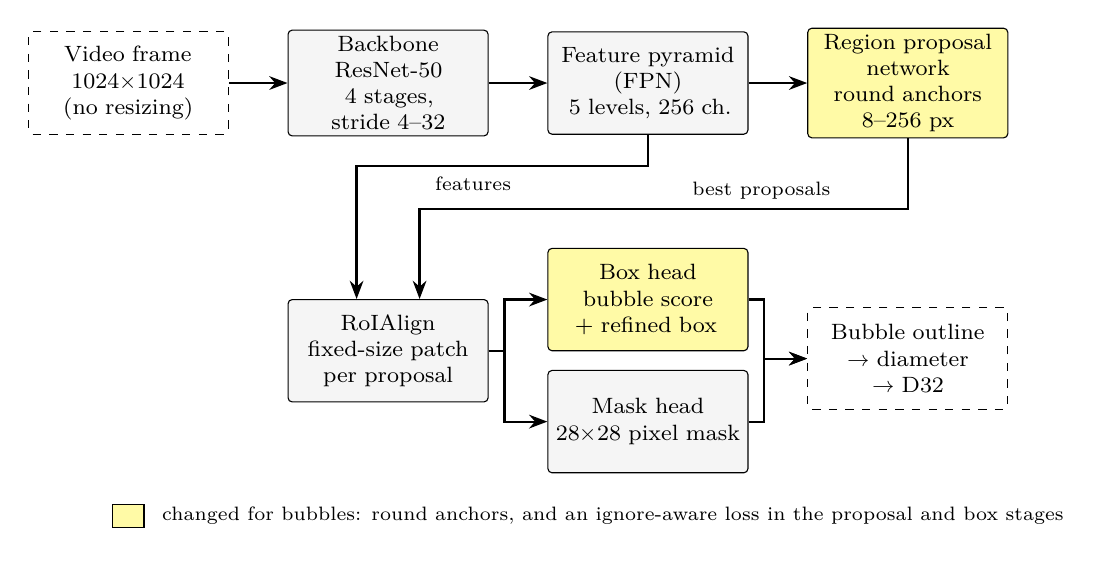
\begin{tikzpicture}[
  font=\footnotesize, >=Stealth,
  blk/.style={draw, rounded corners=1.5pt, align=center, fill=gray!8, minimum height=13mm, text width=24mm, inner sep=2pt},
  mod/.style={blk, fill=yellow!35},
  io/.style={blk, fill=white, dashed},
  arr/.style={->, thick}]
% row 1: features and proposals
\node[io]  (in)  at (0,0)    {Video frame\\1024$\times$1024\\(no resizing)};
\node[blk] (bb)  at (3.3,0)  {Backbone\\ResNet-50\\4 stages, stride 4--32};
\node[blk] (fpn) at (6.6,0)  {Feature pyramid\\(FPN)\\5 levels, 256 ch.};
\node[mod] (rpn) at (9.9,0)  {Region proposal\\network\\round anchors 8--256 px};
% row 2: per-proposal heads
\node[blk] (roi) at (3.3,-3.4) {RoIAlign\\fixed-size patch\\per proposal};
\node[mod] (box) at (6.6,-2.75) {Box head\\bubble score\\+ refined box};
\node[blk] (msk) at (6.6,-4.3) {Mask head\\28$\times$28 pixel mask};
\node[io]  (out) at (9.9,-3.5) {Bubble outline\\$\rightarrow$ diameter\\$\rightarrow$ D32};
\draw[arr] (in) -- (bb); \draw[arr] (bb) -- (fpn); \draw[arr] (fpn) -- (rpn);
\draw[arr] (fpn.south) -- ++(0,-0.4) -| node[pos=0.3, below, font=\scriptsize]{features} ([xshift=-4mm]roi.north);
\draw[arr] (rpn.south) -- ++(0,-0.9) -| node[pos=0.15, above, font=\scriptsize]{best proposals} ([xshift=4mm]roi.north);
\draw[arr] (roi.east) -- ++(2mm,0) |- (box.west);
\draw[arr] (roi.east) -- ++(2mm,0) |- (msk.west);
\draw[arr] (box.east) -- ++(2mm,0) |- (out.west);
\draw[arr] (msk.east) -- ++(2mm,0) |- (out.west);
\node[fill=yellow!35, draw, minimum width=4mm, minimum height=3mm, inner sep=0pt] (k) at (0,-5.5) {};
\node[right=1mm of k, font=\scriptsize, align=left] {changed for bubbles: round anchors, and an ignore-aware loss in the proposal and box stages};
\end{tikzpicture}
\caption{Mask R-CNN as used for pulp bubbles. Shaded: parts changed in this project.}
\label{fig:arch-pulp}
\end{figure}

\begin{enumerate}
\tightlist
\item \textbf{Backbone.} A ResNet-50 convolutional network turns the frame
into feature maps at four scales (1/4 to 1/32 of the frame size). Early
layers respond to edges and textures, deeper layers to larger shapes. It
starts from weights pretrained on COCO, a public dataset of 118,000
everyday photos with hand-outlined objects \citep{lin2014}, so it already
knows general visual features before seeing a bubble (transfer learning).
The first two stages are kept frozen during training.
\item \textbf{Feature pyramid network (FPN).} Combines the deep and shallow
maps so every scale has both detail and context. Small bubbles are found on
the fine levels, large ones on the coarse levels.
\item \textbf{Region proposal network (RPN).} Slides over every pyramid
level and, at each position, scores a set of reference boxes (anchors) for
``contains a bubble'' and adjusts their position and size. The anchors were
changed to round (aspect ratio 1) and bubble-sized, 8--256~px.
\item \textbf{RoIAlign.} Cuts a fixed-size feature patch out of the pyramid
for each of the best proposals, without rounding errors, so a 20~px and a
150~px bubble are both described by the same size of input to the heads.
\item \textbf{Heads.} The box head decides bubble or background and refines
the box; the mask head predicts, for each pixel in the box, whether it
belongs to the bubble. The mask is resized back to the bubble, thresholded
at 0.5, and its area gives the equivalent-area diameter.
\end{enumerate}

Training minimises the sum of five losses: proposal score and box, final
score and box, and mask. In this project, proposals and boxes that fall
mostly inside a hand-drawn ignore region (part-hidden bubbles) are removed
from the background part of these losses, so the network is never taught
that a hidden bubble is empty water. The changes made for bubbles are listed
below.



\begin{longtable}[]{@{}
  >{\raggedright\arraybackslash}p{(\columnwidth - 4\tabcolsep) * \real{0.3333}}
  >{\raggedright\arraybackslash}p{(\columnwidth - 4\tabcolsep) * \real{0.3333}}
  >{\raggedright\arraybackslash}p{(\columnwidth - 4\tabcolsep) * \real{0.3333}}@{}}
\toprule\noalign{}
\begin{minipage}[b]{\linewidth}\raggedright
Component
\end{minipage} & \begin{minipage}[b]{\linewidth}\raggedright
Choice
\end{minipage} & \begin{minipage}[b]{\linewidth}\raggedright
Reason
\end{minipage} \\
\midrule\noalign{}
\endhead
\bottomrule\noalign{}
\endlastfoot
Architecture & torchvision Mask R-CNN, ResNet-50-FPN-v2, COCO-pretrained
\citep{lin2014, li2021} & Instance masks give a per-bubble outline and
so a diameter \\
Input scale & No internal resizing & Resizing breaks the pixel scale and
shrinks small bubbles below the anchors \\
Anchors & Aspect ratio 1 only, 3 sizes per level at $\sqrt{2}$ spacing, 8--256
px & Bubbles are round; worst-case anchor IoU about 0.71 instead of
0.50 \\
Ignore-aware loss & Anchors and proposals mostly inside ignore regions
removed from the background loss & Otherwise part-hidden bubbles train
as background \\
Augmentation & Flips, gamma, scale jitter 0.75--2.0× (p = 0.5) &
Supplies the large-bubble examples the labels lack \\
Training & 512 px random tiles, AdamW \citep{loshchilov2019}, lr 1e-3,
cosine schedule, batch 2, early backbone frozen, CPU & Full frames on a
laptop CPU \\
Checkpoint & Lowest validation loss on the held-out clip (epoch 16 of
20) & Never selected on training loss \\
\end{longtable}

\hypertarget{evaluation}{%
\subsection{Evaluation}\label{evaluation}}

\begin{itemize}
\tightlist
\item
  Split by clip, never by frame: frames within a clip are
  near-duplicates.
\item
  A match needs mask IoU $\geq$ 0.5.
\item
  Diameter is the equivalent-area diameter, d = 2$\surd$(A/$\pi$), for labels and
  predictions alike.
\item
  The headline quantity is the D32 ratio, model D32 divided by hand D32.
\item
  Predictions are matched before any filtering, and the 12 px floor
  applies to predictions too.
\item
  Bubbles cut by the image border are not scored on either side (edge
  rule).
\item
  Only full frames are scored.
\end{itemize}

The detection confidence threshold is 0.40. The inherited tool used
0.72, a value meant to reject murk, which the ignore regions now handle.
Because D32 is volume-weighted, a missed 130 px bubble changes it about
17 times more than a spurious 50 px bubble, so the threshold is set to
favour recall of large bubbles rather than F1. Only these two values
were ever compared, once, on the first September test crops (recall
0.52 vs 0.69, D32 ratio 0.80 vs 0.82). The threshold was then fixed in
the code before the nine full-frame test frames were labelled and before
cross-validation was run, and it was never tuned afterwards. The
full-frame and cross-validation results are therefore free of threshold
selection; the 124-bubble fixed-split figure in Section~6.1 still
contains those 48 September crop bubbles, so the full-frame figure (76
bubbles, D32 ratio 0.96) is the cleaner fixed-split number.

\hypertarget{cross-validation}{%
\subsection{Cross-validation}\label{cross-validation}}

Leave-one-clip-out over the 8 rotor clips: train on 7, test on the 8th,
so every clip is tested once \citep{roberts2017}. The recipe was frozen
beforehand: 12 epochs, confidence 0.40, the same anchors, scale jitter
and edge rule, and the same COCO starting point for every fold. Each
fold took 2.5--3.5 hours on CPU. Results are reported as the mean ± SD
across clips and pooled over bubbles.

\hypertarget{pulp-results}{%
\section{Pulp results}\label{pulp-results}}

The final model sizes bubbles as consistently as a repeat hand label: on
unseen clips its D32 is within 1.5\% of the hand value on average.
Precision against the labels is low, but the audit in 6.3 shows the
labels, not the model, account for most of that gap.

\hypertarget{previous-and-final-model-on-the-same-124-held-out-bubbles}{%
\subsection{Previous and final model on the same 124 held-out
bubbles}\label{previous-and-final-model-on-the-same-124-held-out-bubbles}}

\begin{longtable}[]{@{}llll@{}}
\toprule\noalign{}
& Previous model (7 Sep) & Final model & Human repeatability \\
\midrule\noalign{}
\endhead
\bottomrule\noalign{}
\endlastfoot
Recall & 0.734 & \textbf{0.847} & 0.82 \\
Precision (against labels) & 0.417 & \textbf{0.461} & --- \\
Mean mask IoU & 0.835 & \textbf{0.891} & 0.875 \\
D32 ratio & 0.819 & \textbf{0.957} & 0.96 \\
\end{longtable}

The final model is better on every measure, precision included, so the
recall gain does not come from predicting more. The large-bubble failure
is fixed (Figure~\ref{fig:f_size}): recall on 100--140
px bubbles rose from 0.62 to 0.90. Because D32 weights by volume, that
moved the D32 error from 18\% low to 4\% low. Three changes were made
together (full-frame labels, scale jitter, new anchors), so the gain is
reported as their combined effect.

\begin{figure}[htbp]
\hypertarget{fig:f_size}{%
\centering
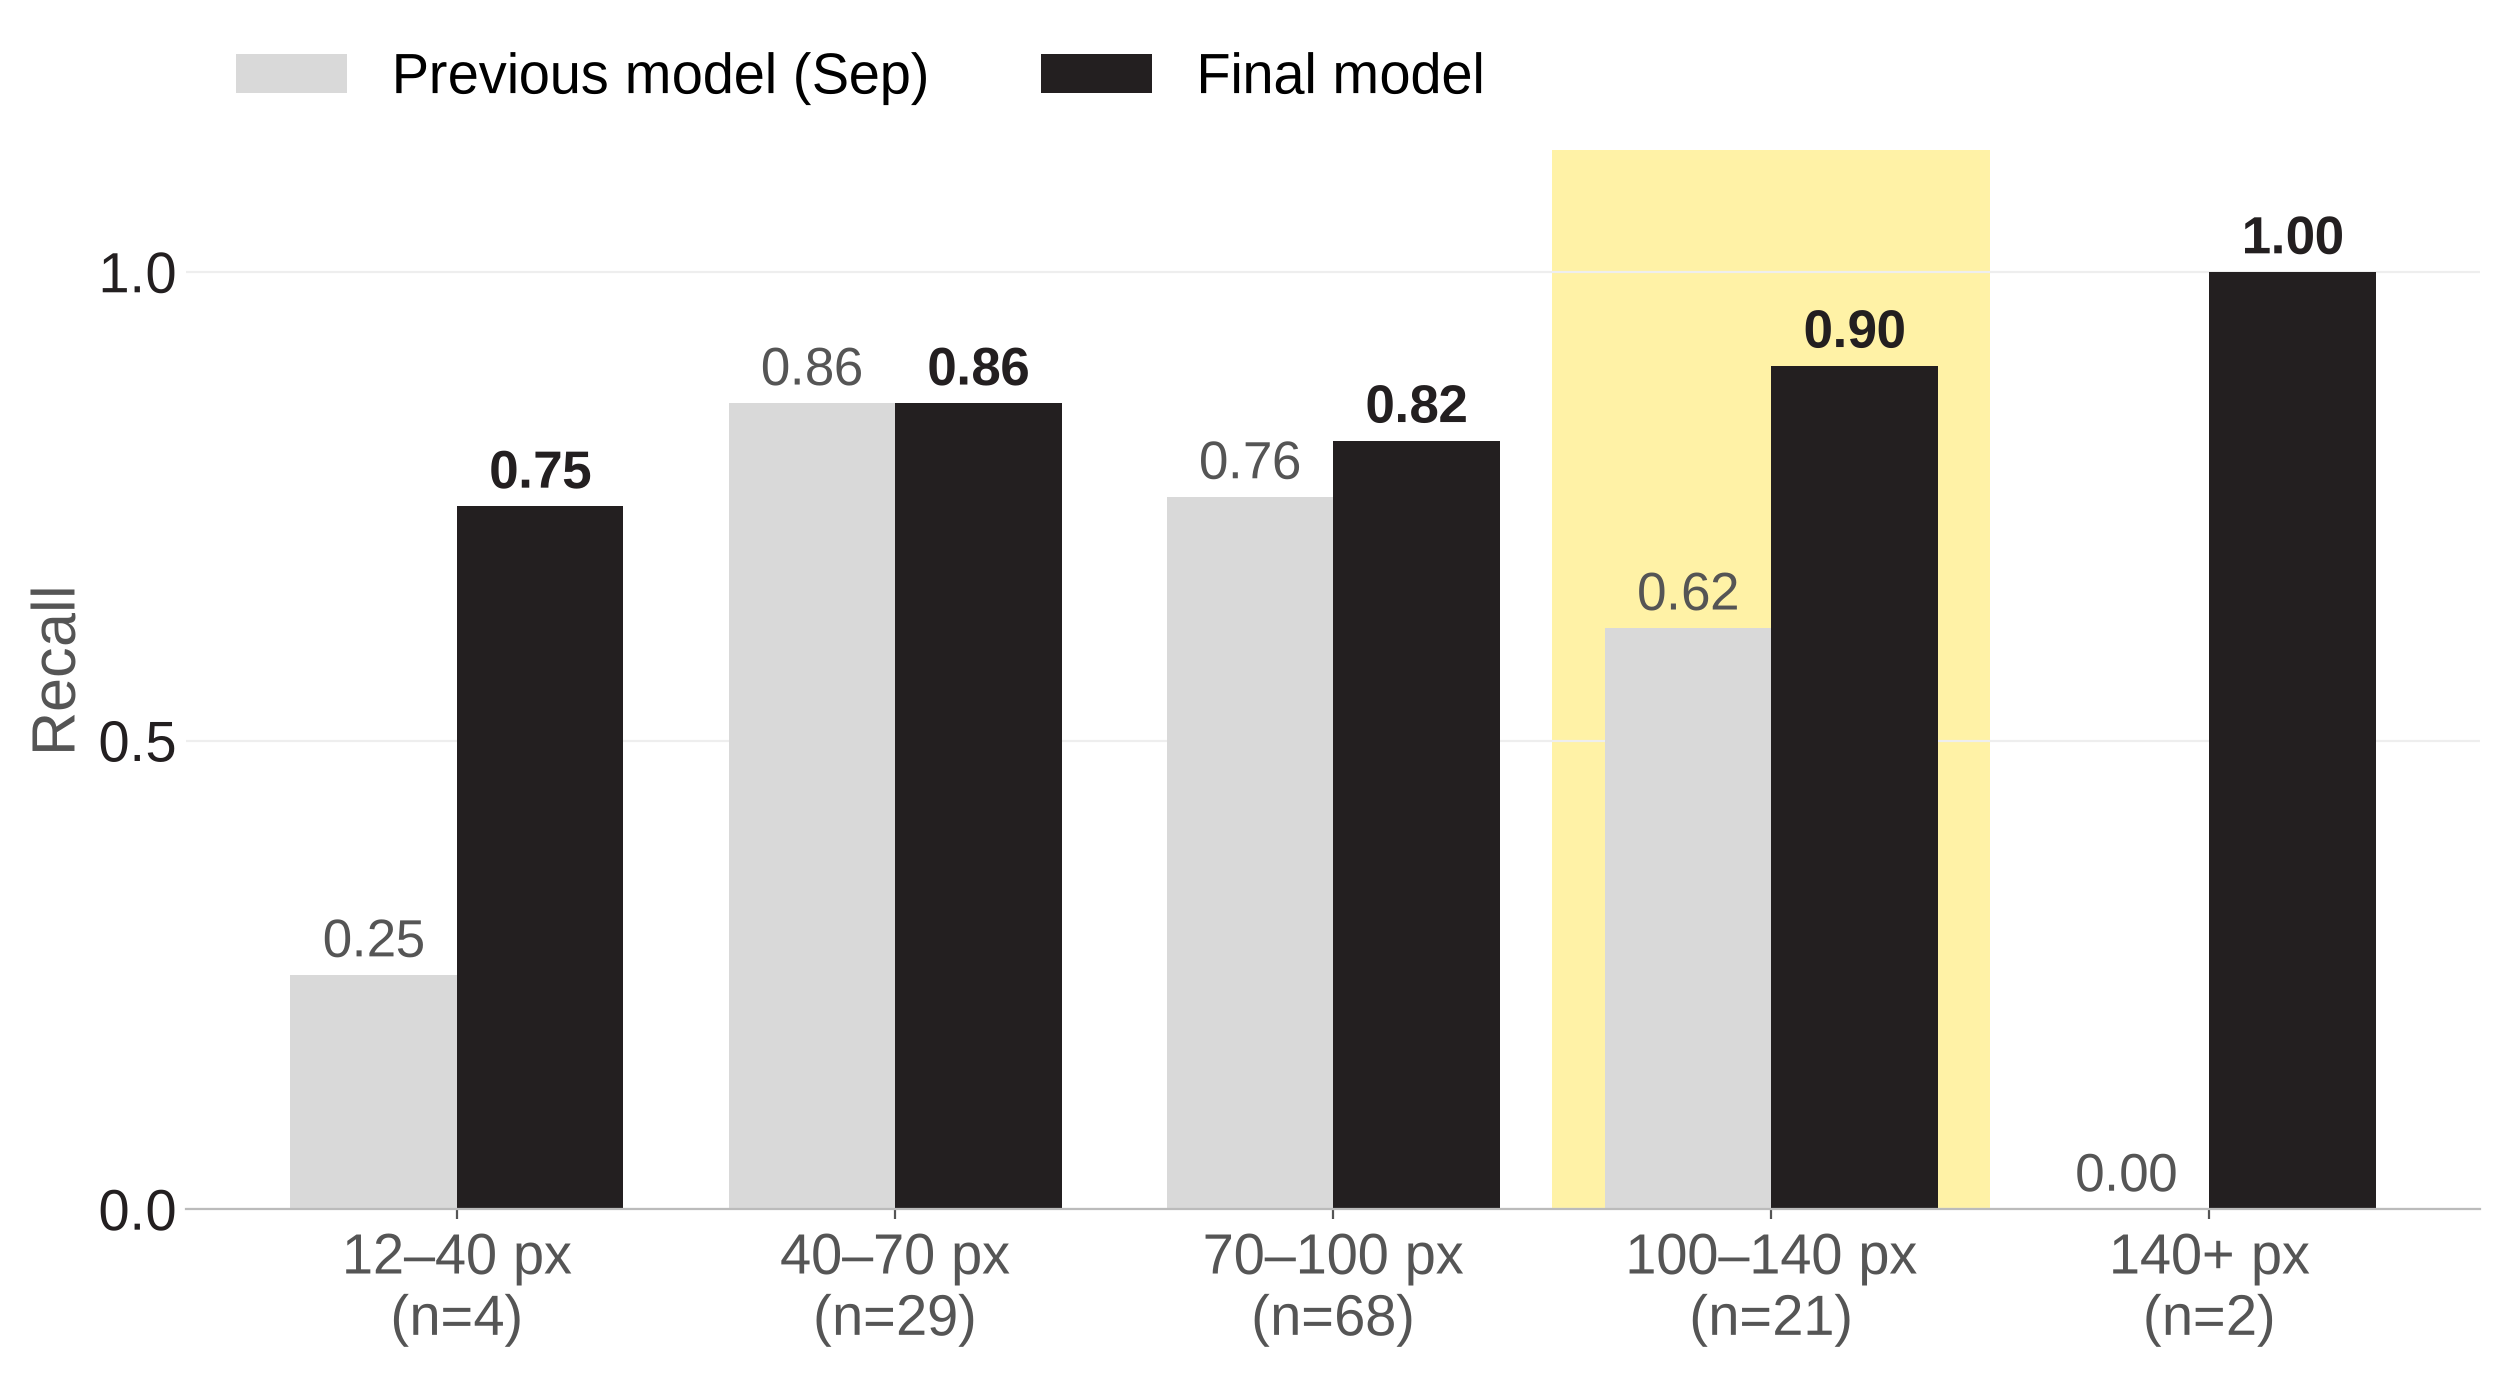
\includegraphics[width=0.82\textwidth]{f_size.png}
\caption{Recall by bubble size, previous vs final model, on the same 124
held-out bubbles. The highlighted band is the size range that moved D32
most.}\label{fig:f_size}
}
\end{figure}

For context, earlier approaches scored far lower on the first test
crops: watershed reached recall 0.03 and a D32 ratio of 0.43; SAM with
automatic masks reached recall 0.52 and a D32 ratio of 0.77, because it
split large bubbles into fragments.

\hypertarget{cross-validation-over-all-8-rotor-conditions}{%
\subsection{Cross-validation over all 8 rotor
conditions}\label{cross-validation-over-all-8-rotor-conditions}}

Across the 8 held-out clips (377 bubbles), recall was 0.921 ± 0.058,
mean mask IoU 0.888 ± 0.011 and the D32 ratio 0.985 ± 0.035. Pooled over
bubbles, recall was 0.910 and the D32 ratio 0.992. The D32 ratio stayed
within 9\% of the hand value on every clip and within 3\% on six of
eight (Figure~\ref{fig:f_cv}). The worst clip was Fine
inline at 0.91. Recall never fell below 0.83 (Med 300air, the smallest
test set).

\begin{figure}[htbp]
\hypertarget{fig:f_cv}{%
\centering
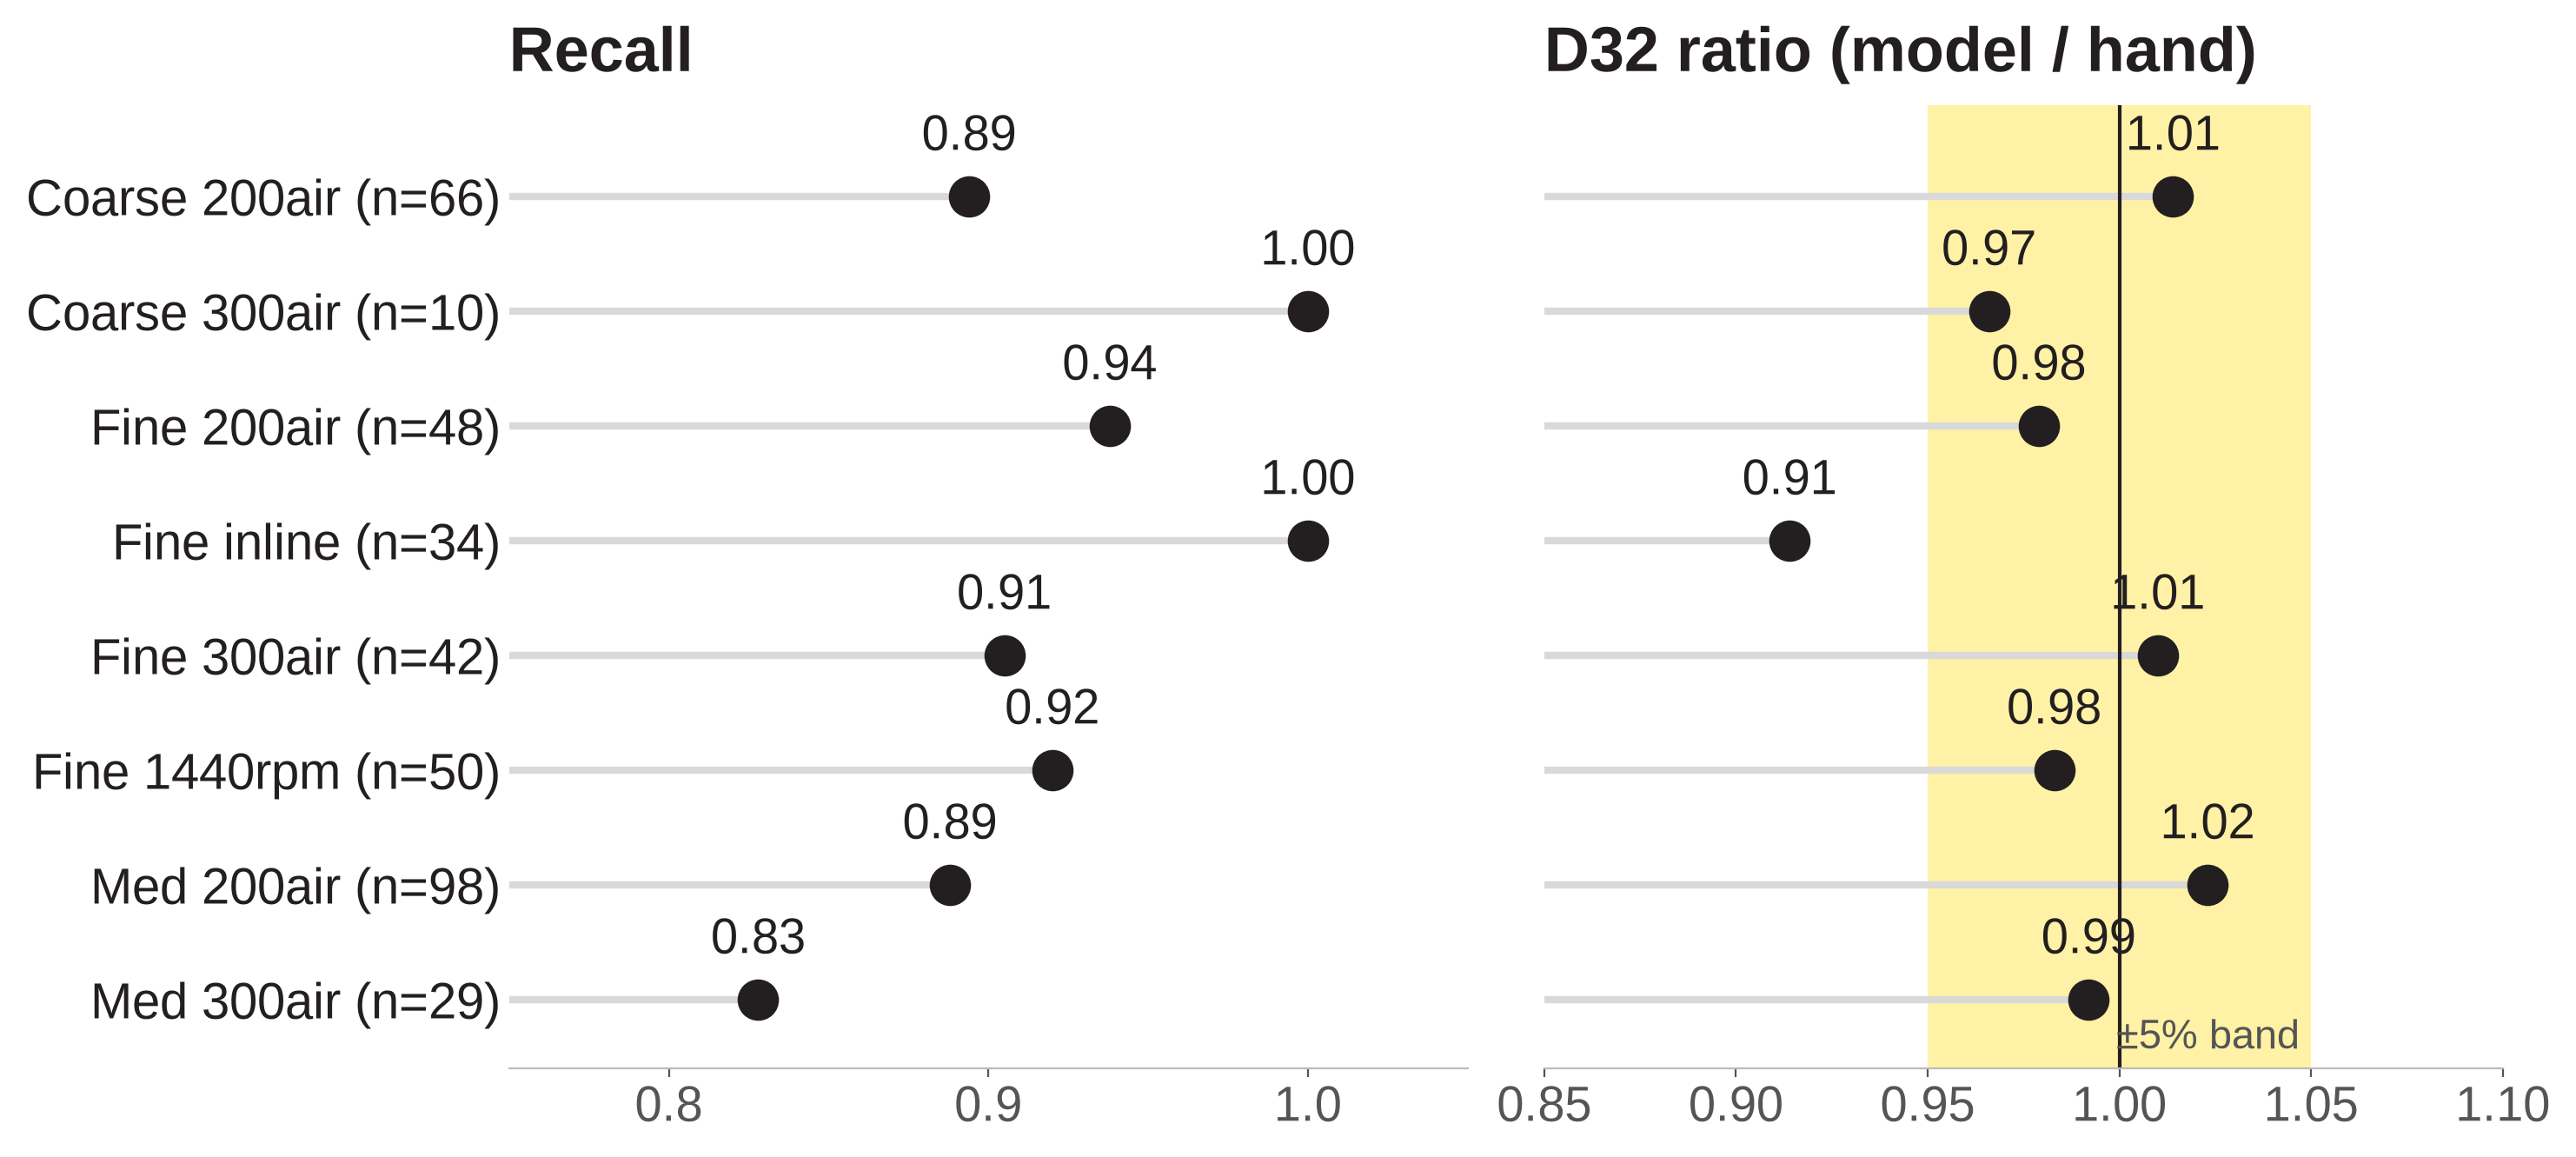
\includegraphics[width=0.82\textwidth]{f_cv.png}
\caption{Leave-one-clip-out results: each clip was held out while the
model trained on the other seven. The shaded band is ±5\% of the
hand-measured D32.}\label{fig:f_cv}
}
\end{figure}

Pooled recall by size was 0.74 for 12--40 px, 0.89 for 40--70 px, 0.93
for 70--100 px and 0.97 for 100--140 px. Precision against labels sat
between 0.38 and 0.50 on every clip (pooled F1 0.60), consistent with
the audit below. The cross-validation figures are higher than the fixed
split because each fold trains on 7 clips instead of 4 and the edge rule
removes truncated bubbles. Both are legitimate differences.

\hypertarget{what-the-false-positives-really-were}{%
\subsection{What the ``false positives'' really
were}\label{what-the-false-positives-really-were}}

All 96 unmatched detections on the 9 test frames were inspected by hand,
with the labels left untouched
(Figure~\ref{fig:f_audit}).

\begin{figure}[htbp]
\hypertarget{fig:f_audit}{%
\centering
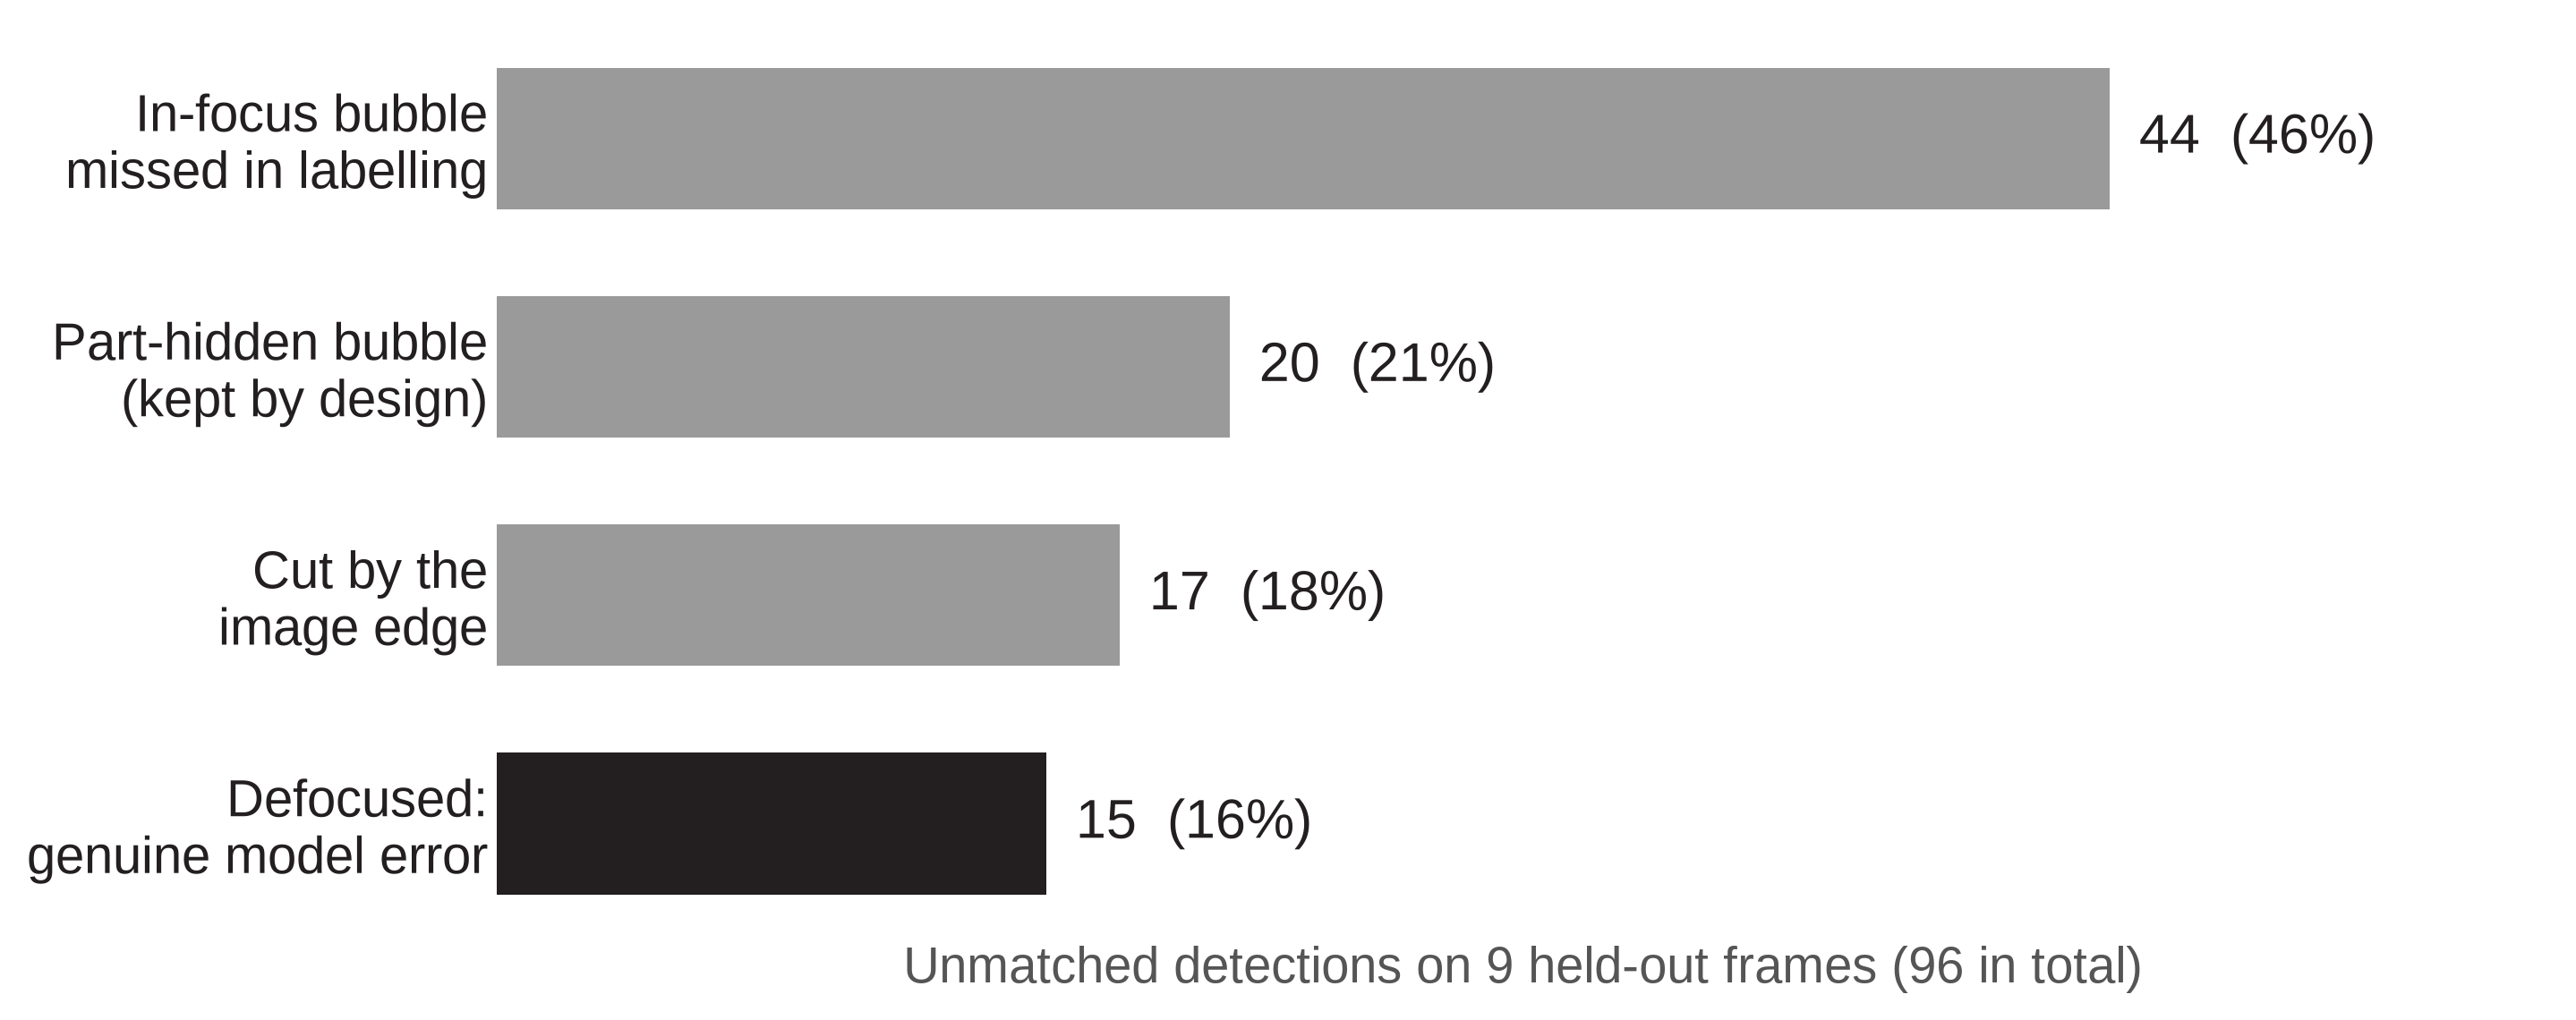
\includegraphics[width=0.82\textwidth]{f_audit.png}
\caption{Hand audit of the 96 detections that matched no label. Only the
defocused group is a genuine model error.}\label{fig:f_audit}
}
\end{figure}

Counting missed in-focus bubbles as correct raises precision from 0.40
to 0.67, and also counting part-hidden bubbles raises it to 0.80. Only
15 of 159 detections (9\%) were real mistakes. A higher confidence
threshold would not help: at 0.8 it removes 11 of the 15 defocused
errors but also 16 of the 44 real bubbles.

\begin{figure}[htbp]
\hypertarget{fig:pulp_gt_vs_model}{%
\centering
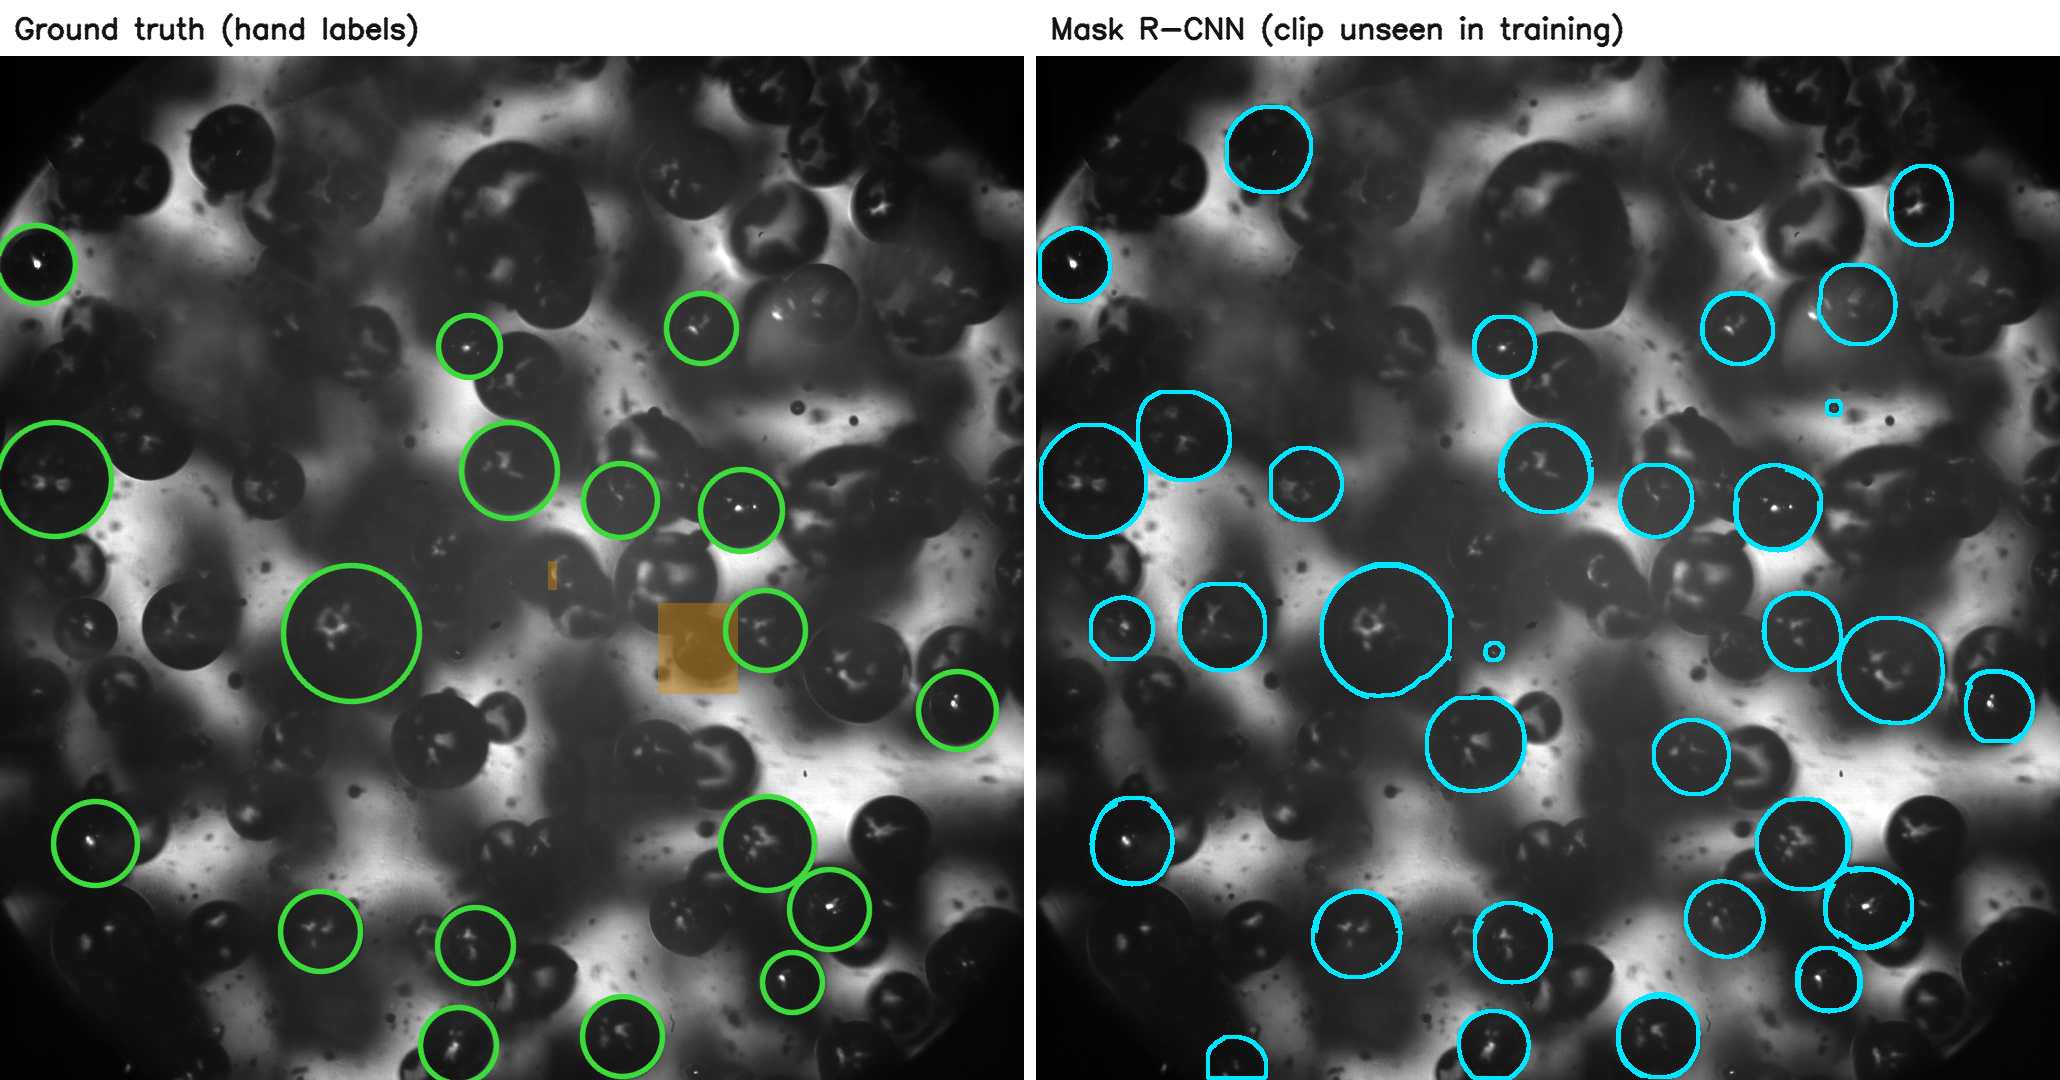
\includegraphics[width=0.95\textwidth]{pulp_gt_vs_model.png}
\caption{Hand labels (left) and model outlines (right) on Fine inline
frame 23, a clip held out in cross-validation. Most extra model outlines
are sharp bubbles that were not labelled.}\label{fig:pulp_gt_vs_model}
}
\end{figure}

\hypertarget{how-many-bubbles-are-enough}{%
\subsection{How many bubbles are
enough?}\label{how-many-bubbles-are-enough}}

D32's 95\% confidence interval is estimated by the delta method for a
ratio, taking the larger of a bubble-level and a frame-level (clustered)
error. A measurement counts as stable when the interval is within ±5\%
of D32, from at least 3 frames, at two frames in a row. On the RotMed
300air clip, D32 was stable after 137 bubbles from 8 frames (254.8
\textmu m ±4.7\%). The Venturi 500 air, 60 ppm clip was not stable after
all 21 sampled frames (355 bubbles, 446 \textmu m ±9.7\%); the model was
never trained on Venturi footage.

\hypertarget{froth-segmentation}{%
\section{Froth segmentation}\label{froth-segmentation}}

Cellpose-SAM, used zero-shot with default settings, finds froth bubbles
reliably and gives a stable D32 of 2.16 mm. Froth is a different problem
from pulp: the bubbles are packed edge to edge, so the task is
separating neighbours rather than finding isolated objects.

\hypertarget{method}{%
\subsection{Method}\label{method}}

\textbf{How Cellpose works.} Cellpose \citep{stringer2021} was designed to
separate touching cells in microscope images, which is the same problem as
separating packed froth bubbles. Instead of drawing boxes, it predicts for
every pixel which way to move to reach the centre of the object it belongs
to (Figure~\ref{fig:arch-froth}).

\begin{figure}[htbp]
\centering
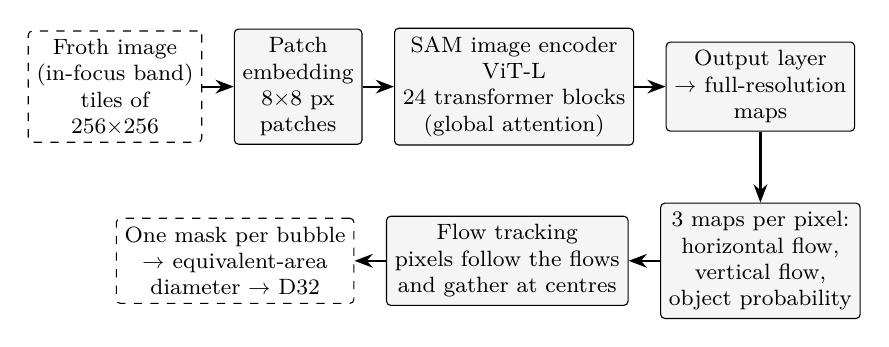
\begin{tikzpicture}[
  font=\footnotesize, >=Stealth, node distance=4mm,
  blk/.style={draw, rounded corners=1.5pt, align=center, fill=gray!8, minimum height=10mm, inner sep=3pt},
  io/.style={blk, fill=white, dashed},
  arr/.style={->, thick}]
\node[io] (in) {Froth image\\(in-focus band)\\tiles of\\256$\times$256};
\node[blk, right=of in] (pe) {Patch\\embedding\\8$\times$8 px\\patches};
\node[blk, right=of pe] (vit) {SAM image encoder\\ViT-L\\24 transformer blocks\\(global attention)};
\node[blk, right=of vit] (head) {Output layer\\$\rightarrow$ full-resolution\\maps};
\node[blk, below=9mm of head] (maps) {3 maps per pixel:\\horizontal flow,\\vertical flow,\\object probability};
\node[blk, left=of maps] (dyn) {Flow tracking\\pixels follow the flows\\and gather at centres};
\node[io, left=of dyn] (out) {One mask per bubble\\$\rightarrow$ equivalent-area\\diameter $\rightarrow$ D32};
\draw[arr] (in) -- (pe); \draw[arr] (pe) -- (vit); \draw[arr] (vit) -- (head);
\draw[arr] (head) -- (maps); \draw[arr] (maps) -- (dyn); \draw[arr] (dyn) -- (out);
\end{tikzpicture}
\caption{Cellpose-SAM as used for froth bubbles, with default settings and no froth training.}
\label{fig:arch-froth}
\end{figure}

\begin{enumerate}
\tightlist
\item \textbf{Encoder.} Cellpose-SAM \citep{pachitariu2025} replaces the
original Cellpose U-Net with the image encoder of Segment Anything
\citep[SAM,][]{kirillov2023}, a vision transformer (ViT-L) pretrained on
about one billion object masks. The image is split into 8$\times$8~px
patches, and the transformer blocks let every patch compare itself with
every other patch in the tile. SAM's own prompt and mask decoders are
removed.
\item \textbf{Outputs.} For every pixel the network predicts a horizontal
and a vertical flow (a small arrow pointing towards the centre of the
object) and the probability that the pixel belongs to any object.
\item \textbf{Flow tracking.} Pixels with high probability are moved step
by step along the arrows. Pixels that end up at the same point form one
object, so two bubbles that touch are still split along the wall between
them. Masks whose flows are inconsistent are discarded.
\end{enumerate}

The released model was trained on about 23,000 microscope images with 3.3
million outlined cells \citep{pachitariu2025}. It was used here exactly as
released, which is why froth measurement needed no labelled froth training
data.



\textbf{Measurement settings.}

\begin{itemize}
\tightlist
\item
  Cellpose-SAM (model cpsam\_v2, cellpose 4.2.1.1), default settings, no
  froth training and nothing tuned.
\item
  Only the in-focus band of each frame is measured, found automatically
  (for example 489 × 424 px at t = 0 s).
\item
  Scale from the 55 mm inner tube width, measured on every frame
  (Section~3.2).
\item
  Same rules as pulp: edge rule, equivalent-area diameter, matching at
  mask IoU $\geq$ 0.5.
\item
  Ground truth: hand-drawn outlines; unresolved areas marked unsure and
  not scored.
\end{itemize}

\begin{figure}[htbp]
\hypertarget{fig:froth}{%
\centering
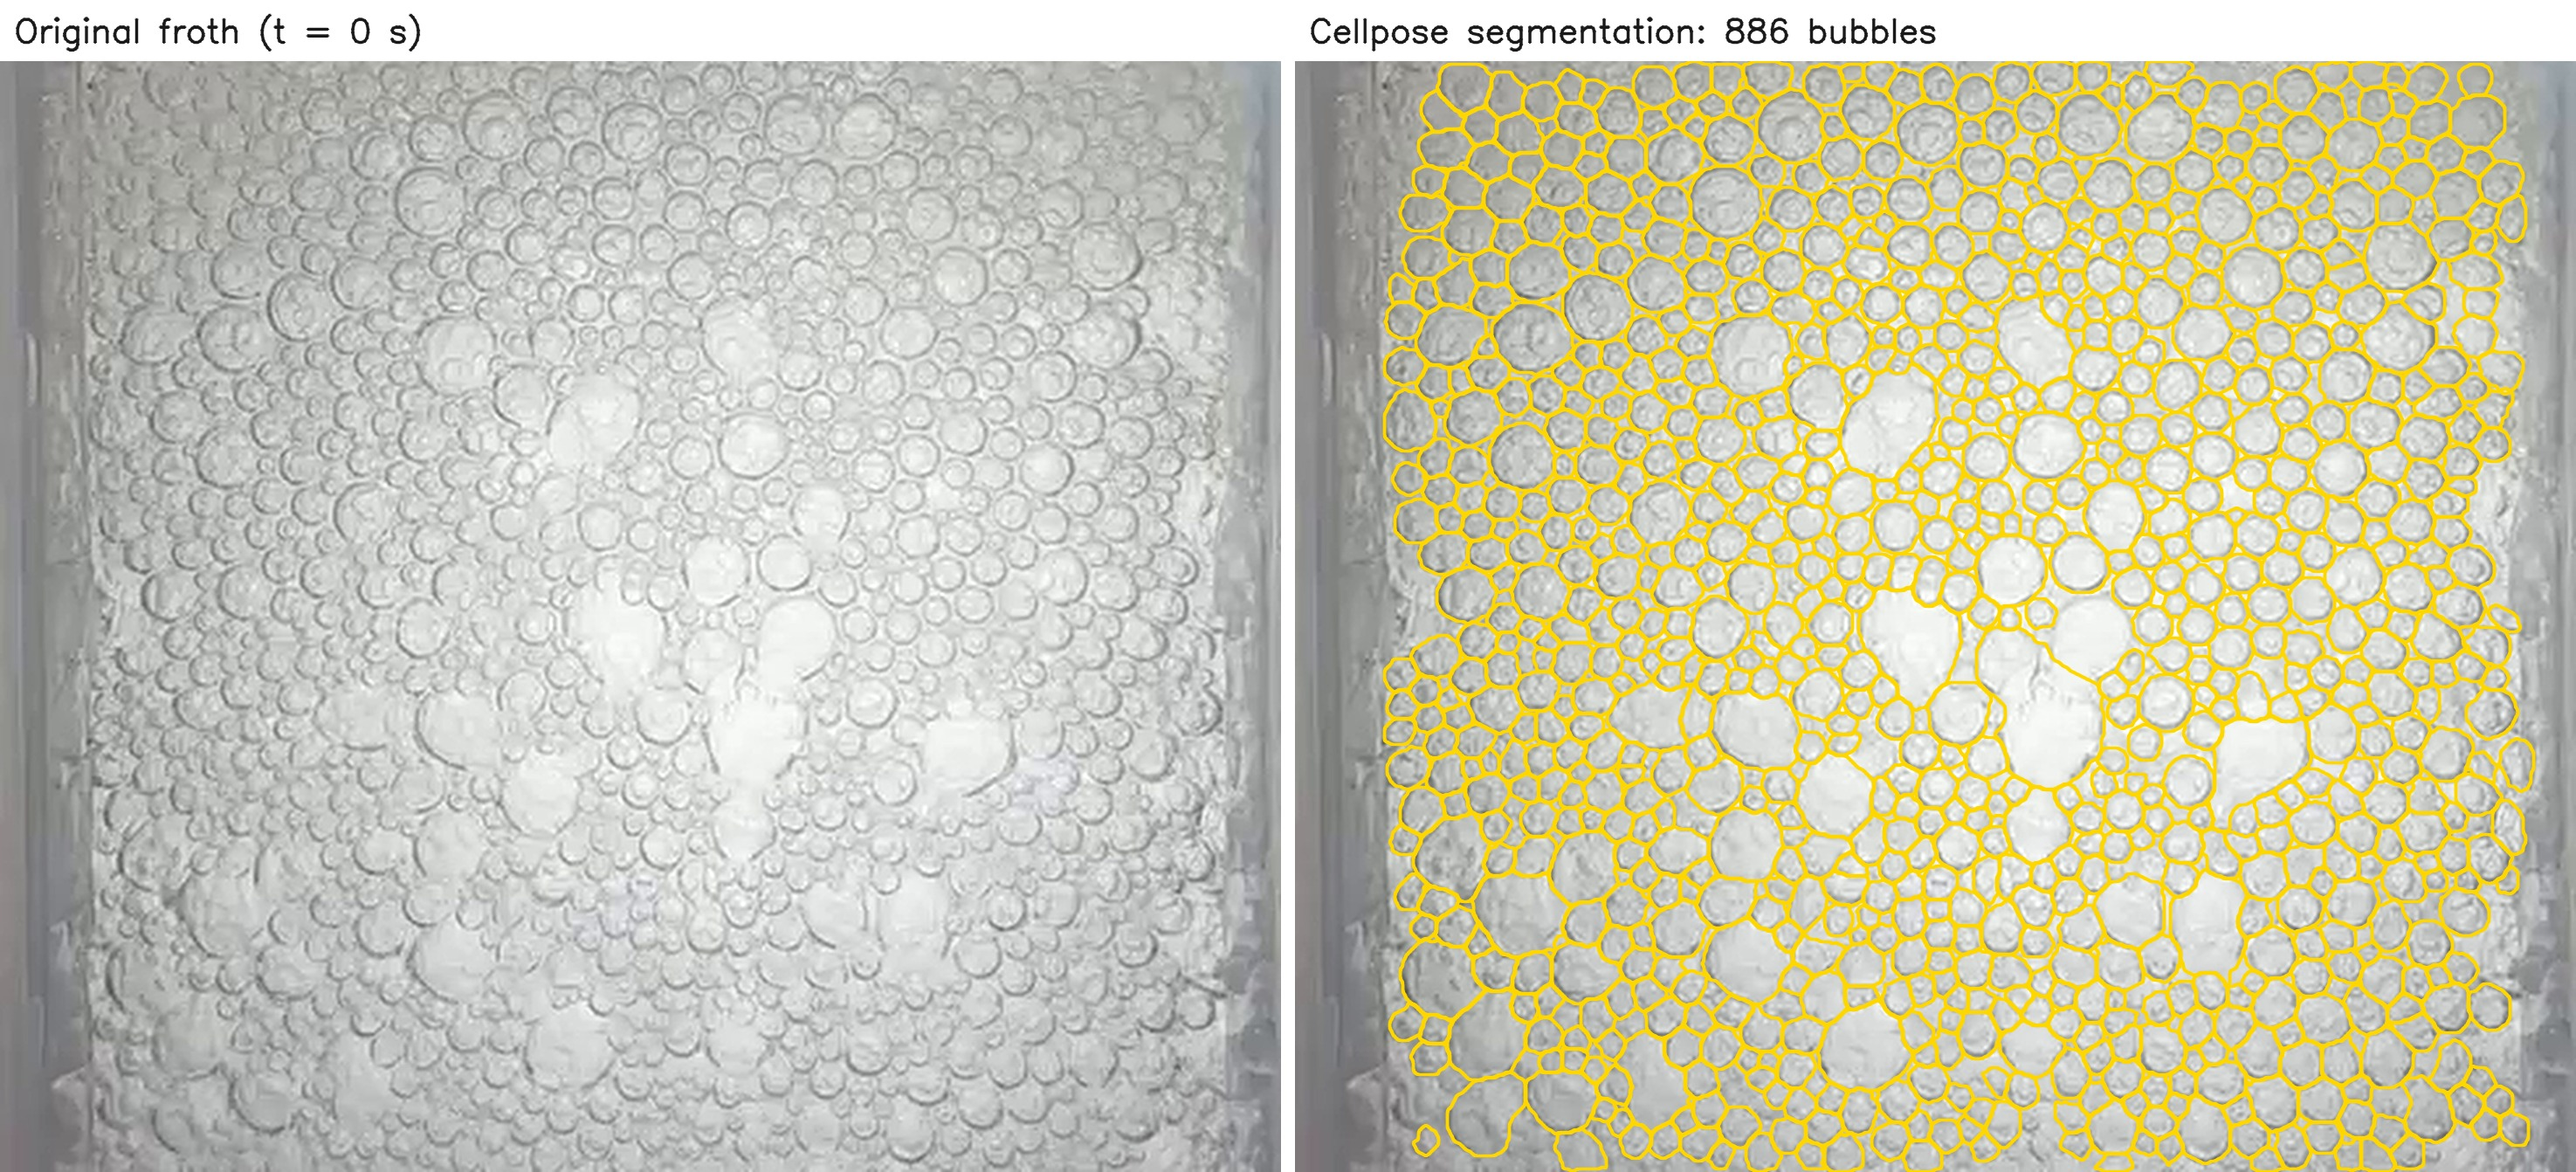
\includegraphics[width=0.95\textwidth]{froth.jpg}
\caption{Froth frame at t = 0 s (left) and Cellpose outlines in the
in-focus band (right), 886 bubbles, no froth training.}\label{fig:froth}
}
\end{figure}

\hypertarget{accuracy-against-hand-labels}{%
\subsection{Accuracy against hand
labels}\label{accuracy-against-hand-labels}}

\begin{longtable}[]{@{}
  >{\raggedright\arraybackslash}p{(\columnwidth - 10\tabcolsep) * \real{0.1667}}
  >{\raggedright\arraybackslash}p{(\columnwidth - 10\tabcolsep) * \real{0.1667}}
  >{\raggedright\arraybackslash}p{(\columnwidth - 10\tabcolsep) * \real{0.1667}}
  >{\raggedright\arraybackslash}p{(\columnwidth - 10\tabcolsep) * \real{0.1667}}
  >{\raggedright\arraybackslash}p{(\columnwidth - 10\tabcolsep) * \real{0.1667}}
  >{\raggedright\arraybackslash}p{(\columnwidth - 10\tabcolsep) * \real{0.1667}}@{}}
\toprule\noalign{}
\begin{minipage}[b]{\linewidth}\raggedright
Test
\end{minipage} & \begin{minipage}[b]{\linewidth}\raggedright
Bubbles
\end{minipage} & \begin{minipage}[b]{\linewidth}\raggedright
Recall
\end{minipage} & \begin{minipage}[b]{\linewidth}\raggedright
Precision
\end{minipage} & \begin{minipage}[b]{\linewidth}\raggedright
Mean IoU
\end{minipage} & \begin{minipage}[b]{\linewidth}\raggedright
D32 ratio
\end{minipage} \\
\midrule\noalign{}
\endhead
\bottomrule\noalign{}
\endlastfoot
Fully labelled patch, t = 240 s & 51 & 0.86 (95\% CI 0.74--0.93) & 0.98
local / 0.68 strict & 0.67 & 1.10 \\
Partly labelled crop, frame 299 & 26 & 1.00 (0.87--1.00) & not
computable & 0.80 & 0.97 \\
\end{longtable}

Every labelled bubble on the patch is at least 80\% covered by its own
Cellpose mask. The 7 counted as missed are 6.6--10 px bubbles whose
Cellpose mask is larger, so IoU falls below 0.5. Strict precision counts
every unlabelled detection as an error; most of those are real bubbles
in the unresolved area, so local precision (unresolved area ignored) is
the fairer figure.

There is a constant boundary offset of +1.2 px in radius: the labels
were traced on the bright cap, while Cellpose places the edge mid-film.
It matters most for small bubbles (diameter ratio 1.31 under 9 px, 1.05
over 17 px). With the labels grown by 1 px, all 51 match, IoU rises to
0.77 and the diameter ratio to 1.08. This is a labelling convention to
settle, not a detection error.

The earlier froth approaches were weaker on the same crop: watershed
(bubseg) found 13 of 26 bubbles, and tiled SAM (BubSAM3) found 23 of 26
with IoU 0.71 at 27--40 minutes per frame.

\hypertarget{consistency-over-the-video}{%
\subsection{Consistency over the
video}\label{consistency-over-the-video}}

\begin{figure}[htbp]
\hypertarget{fig:f_froth}{%
\centering
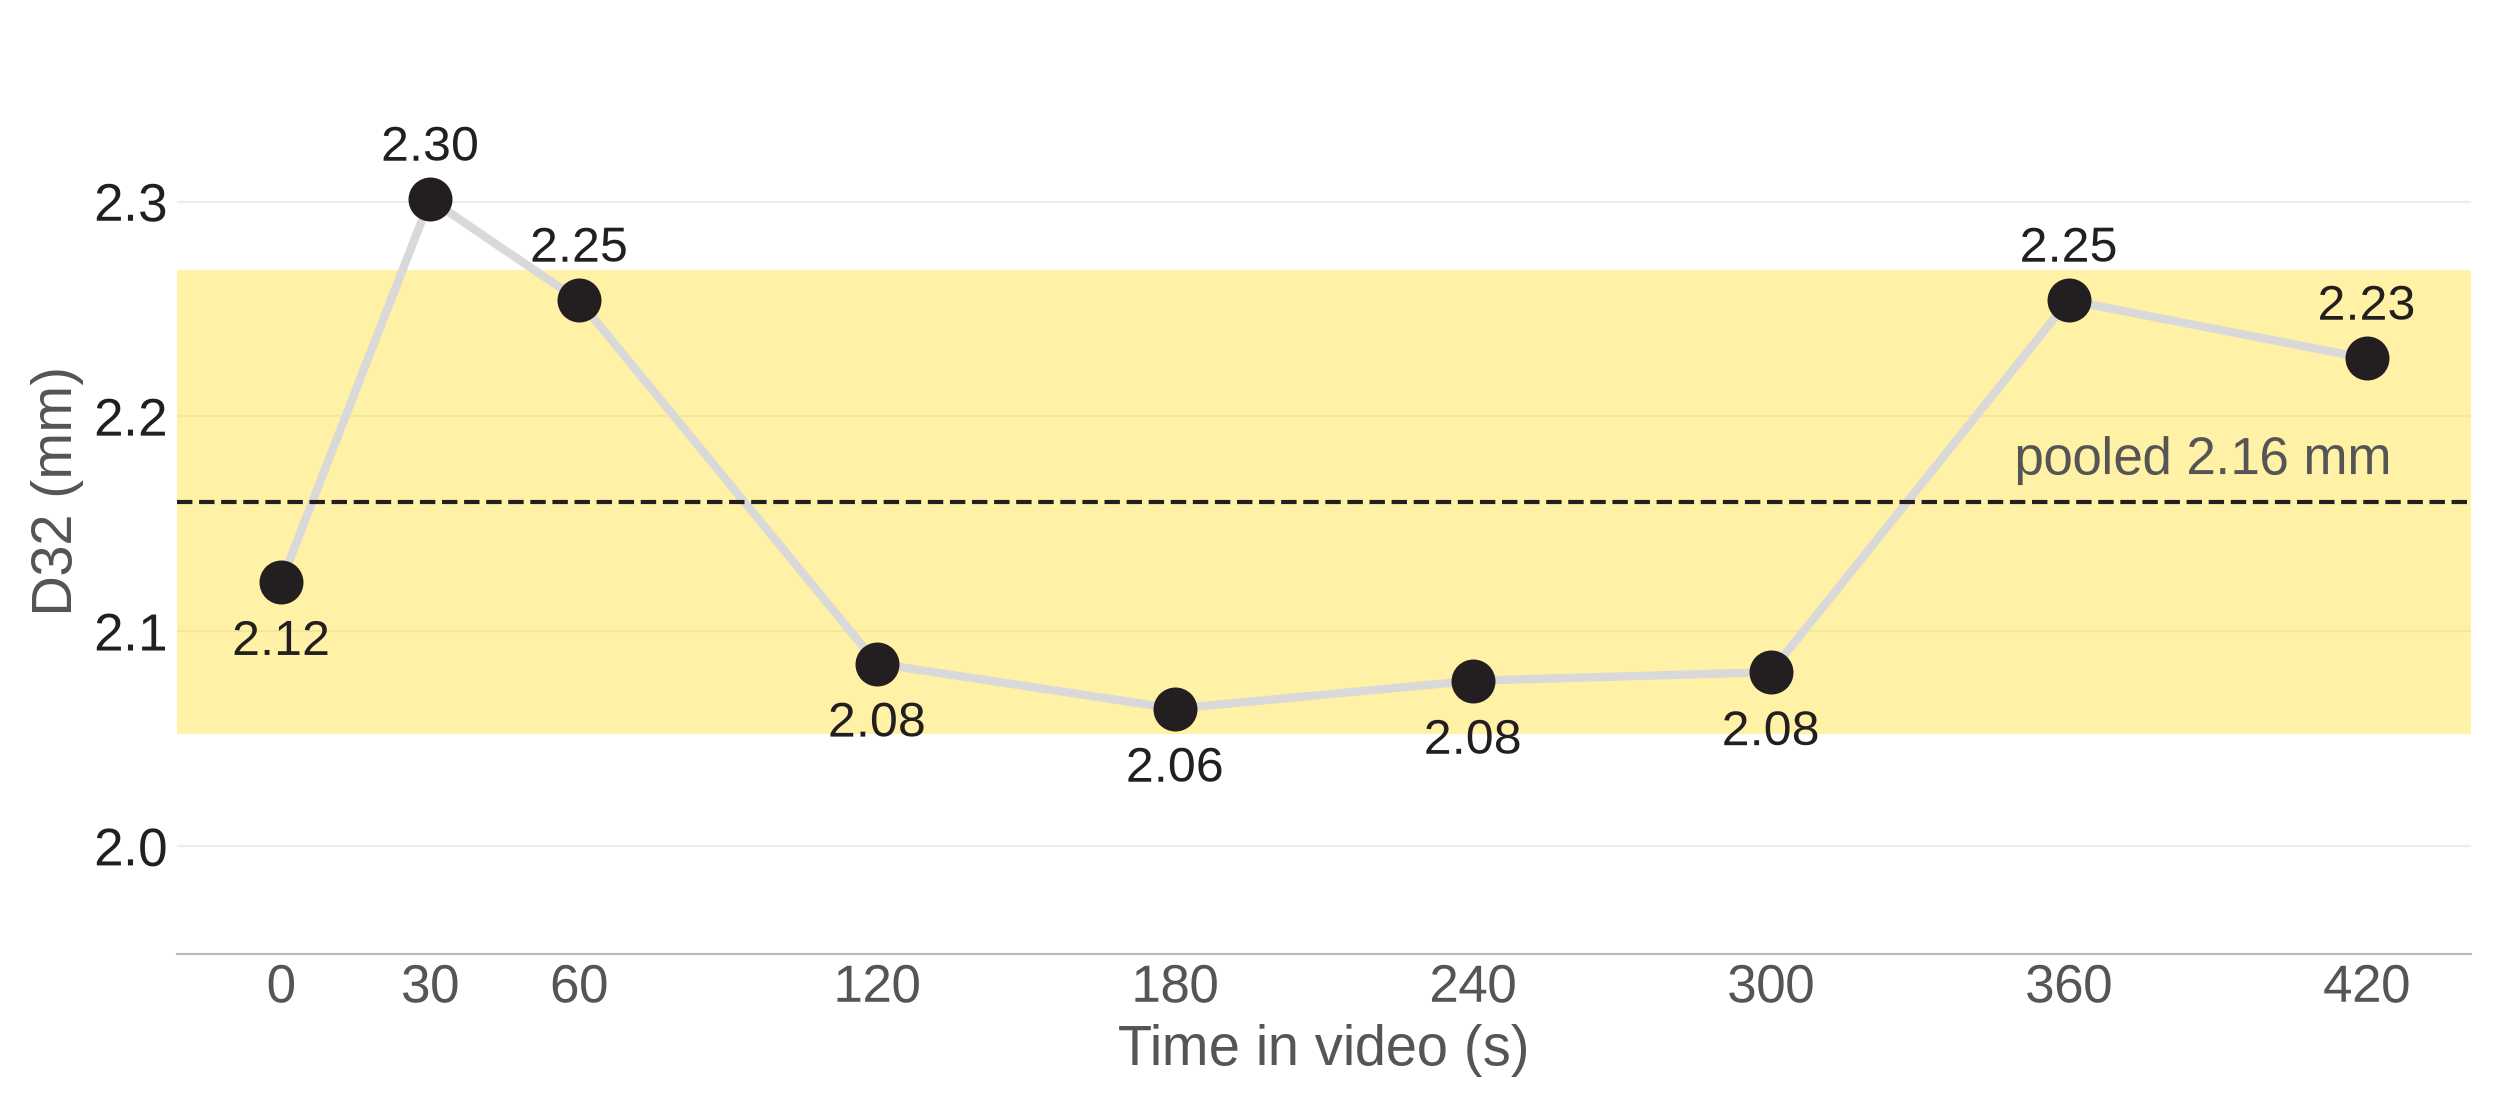
\includegraphics[width=0.82\textwidth]{f_froth.png}
\caption{Froth D32 on 9 frames spread over 7 minutes (6,075 bubbles).
The dashed line is the pooled D32; the shaded band is ±5\% of
it.}\label{fig:f_froth}
}
\end{figure}

Over 9 frames spread across 7 minutes, the pooled D32 is 2.16 mm and
every frame lies within 2.06--2.30 mm. Cellpose takes 30--48 s per frame
on a laptop CPU, 35--80 times faster than tiled SAM.

A bootstrap over the pooled bubbles puts the 95\% interval at ±11\% for
200 bubbles, ±5\% for about 1,100 and ±2.1\% for all 6,075.
Frame-to-frame spread (4.4\%) is slightly above what sampling alone
explains (3.2\%, p = 0.08), so the stopping rule also uses a frame-level
interval. In the order the software visits frames, it stops after 6--7
frames with D32 within 2\% of the 9-frame value. A whole t = 150 s frame
with 160 more hand outlines is ready to score; it needs one Cellpose run
on that frame.

\hypertarget{software-bubblemetrix}{%
\section{Software: BubbleMetrix}\label{software-bubblemetrix}}

BubbleMetrix wraps both pipelines in a Windows desktop app so a
researcher picks a video and presses one button. It runs on a laptop CPU
with no settings to tune; the user manual covers installation and every
feature.

\begin{figure}[htbp]
\hypertarget{fig:gui}{%
\centering
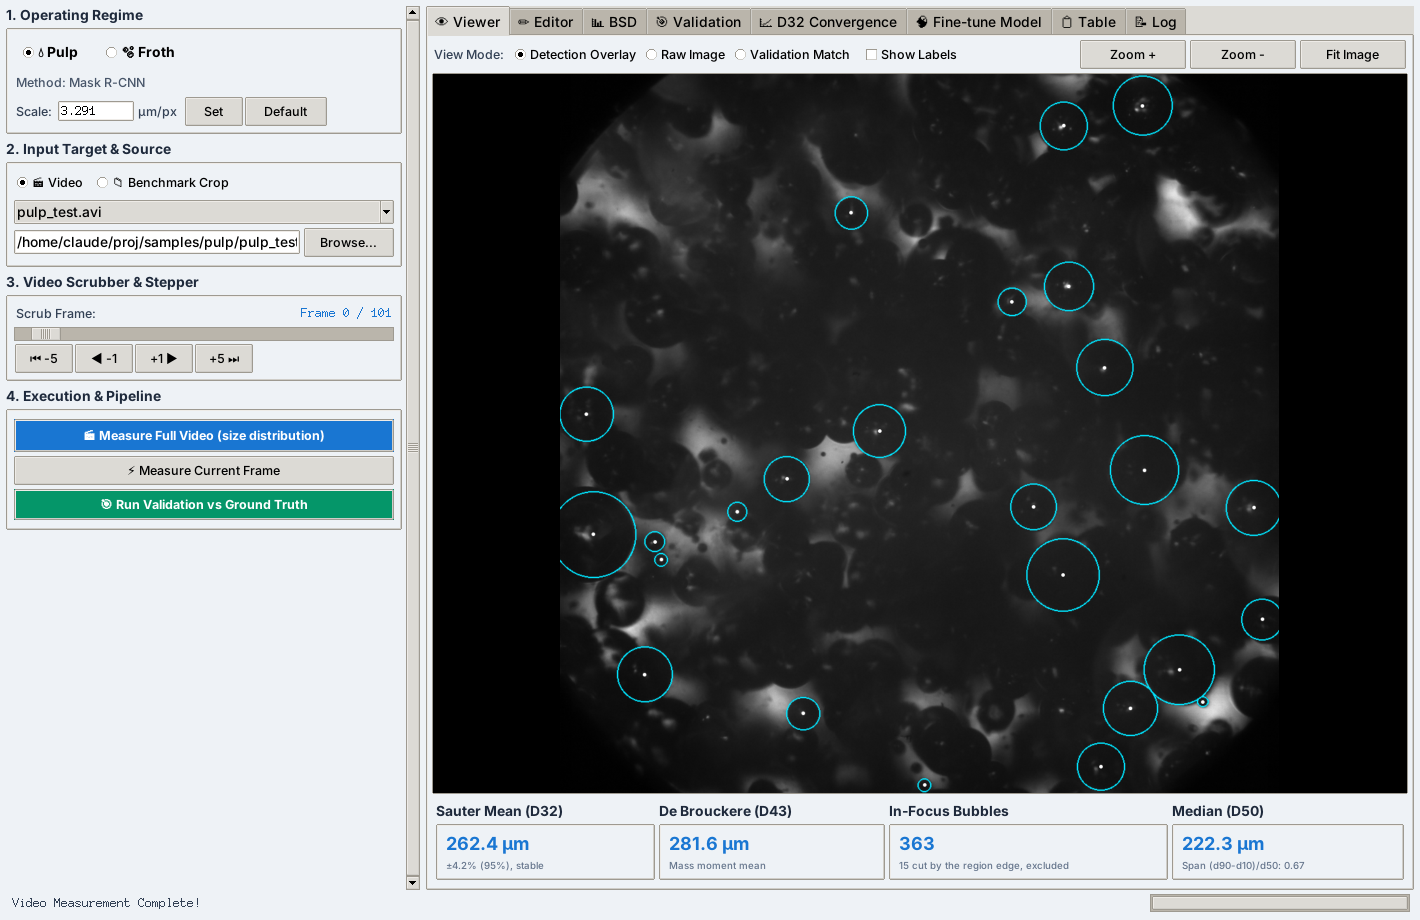
\includegraphics[width=0.95\textwidth]{gui.png}
\caption{BubbleMetrix after measuring a pulp clip: outlines on the
current frame, and D32 with its 95\% interval in the result
cards.}\label{fig:gui}
}
\end{figure}

\begin{longtable}[]{@{}
  >{\raggedright\arraybackslash}p{(\columnwidth - 2\tabcolsep) * \real{0.5000}}
  >{\raggedright\arraybackslash}p{(\columnwidth - 2\tabcolsep) * \real{0.5000}}@{}}
\toprule\noalign{}
\begin{minipage}[b]{\linewidth}\raggedright
Feature
\end{minipage} & \begin{minipage}[b]{\linewidth}\raggedright
What it does
\end{minipage} \\
\midrule\noalign{}
\endhead
\bottomrule\noalign{}
\endlastfoot
Pulp or froth & Mask R-CNN for pulp; Cellpose for froth, run in its own
environment through a helper process. Settings are fixed at their
validated values. \\
Scale & Adjustable. Pulp default 3.291 \textmu m/px; froth measured from
the 55 mm inner tube width on every frame. Changing it re-expresses
results without re-running detection. \\
Measure Full Video & Pulp: every frame outlined, D32 from every 5th
frame (bubbles repeat between consecutive frames). Froth: up to 40
frames spread over the clip, stopping once D32 is stable. \\
D32 Convergence & Running D32 with its 95\% band against bubbles
measured, and either ``stable after N bubbles'' or an estimate of how
many more are needed. \\
Editor and Validation & Correct detections by hand; score the model
against hand labels (recall, precision, IoU, D32 ratio). \\
Fine-tune Model & Add frames from new footage, correct the model's
suggestions, see the current model's accuracy, then fine-tune in the
background (30--60 min on CPU). The new model is used only if it beats
the old one on held-back frames and is no worse on a fixed benchmark;
one click reverts. \\
Exports & CSV per bubble (with frame number) and a JSON summary
including the convergence result. \\
\end{longtable}

The fine-tuning minimums are 15 frames and 150 bubbles for pulp, and 4
boxes and 300 bubbles for froth. The froth figure follows Cellpose 2.0,
where 100--200 corrected objects suffice when the model pre-labels the
images \citep{pachitariu2022}. The pulp figure comes from this project's
own runs: 65 labelled bubbles gave recall 0.52, while about 330 per
cross-validation fold gave 0.91. Both are floors; the held-back
comparison decides.

\subsection{When is fine-tuning needed?}\label{when-finetune}

Fine-tuning is a safety net rather than a routine step. What decides it
is whether the \emph{images} look different from those the model was
validated on, not whether the operating condition is new.

\textbf{Froth.} Cellpose is used without froth training, so a new
operating condition is not new to it in the way it would be for a trained
model. As a first check, nine further froth videos from the same rig were
compared with the validated 180WW video using simple image statistics in
the in-focus band: mean brightness, edge contrast (standard deviation of
the high-pass image) and bubble spacing (first peak of its
autocorrelation), averaged over frames at 60, 180, 300 and 420~s
(Table~\ref{tab:newfroth}). These are not segmentation results.

\begin{table}[htbp]
\centering
\small
\caption{Image statistics of the new froth videos against the validated
video (180WW). Spacing is in pixels and tracks bubble size: 16--17~px for
180WW matches its measured D32 of about 18~px.}
\label{tab:newfroth}
\begin{tabular}{@{}lrrrl@{}}
\toprule
Video & Brightness & Edge contrast & Spacing (px) & vs 180WW \\
\midrule
180WW (validated) & 185 & 13.9 & 16--17 & reference \\
30WW & 186 & 14.0 & 16--17 & same \\
90WW & 184 & 14.2 & 16--17 & same \\
Repeat 2 & 182 & 13.7 & 15--17 & same \\
Repeat 1 & 183 & 13.0 & 16--18 & same \\
60WW & 192 & 12.7 & 14--20 & close \\
Baseline & 179 & 12.5 & 17--18 & close \\
Paddle 20 rpm & 183 & 12.1 & 16--17 & close \\
Paddle 40 rpm & 192 & 11.7 & 17--18 & close \\
\textbf{Paddle 6 rpm} & \textbf{173} & \textbf{8.7} & \textbf{18--24} & \textbf{different} \\
\bottomrule
\end{tabular}
\end{table}

Nine of the ten videos match the validated footage closely, so zero-shot
Cellpose is expected to carry over. Paddle 6~rpm has larger bubbles and
about 37\% less wall contrast, and is the first condition to check.

\textbf{Pulp.} The pulp model is trained, but cross-validation already
tested it on rotor conditions it had not seen (D32 ratio $0.99\pm0.03$).
New rotor conditions on the same probe and lighting should not need
retraining. Footage that looks different does: the over-exposed Venturi
and diluted clips, or a new camera, lens or magnification.

The recommended workflow is therefore: measure the new footage, check one
small hand-labelled patch (or a couple of frames) per new condition, and
fine-tune only if that check fails. The labels made for the check are the
same ones fine-tuning would use, so no effort is wasted.

\hypertarget{discussion}{%
\section{Discussion}\label{discussion}}

\textbf{Sizing matches a human; selection is the open question.} Mask
IoU (0.89) and the D32 ratio (0.96 fixed split, 0.99 cross-validated)
sit at the level of two hand-labelling passes by the same person (0.875
and 0.96). Where model and labels disagree, it is about which bubbles
count, exactly as the repeatability study predicted.

\textbf{The model exposed a labelling bias.} On full 1024 px frames,
small or faint bubbles with a clear edge were easy to skip. The model,
trained only on in-focus round bubbles, found them anyway, which
suggests it learned what a bubble looks like rather than copying the
annotator. The standard fix is a blind completeness pass over the labels
followed by retraining.

\textbf{Part-hidden bubbles are included on purpose.} The labels exclude
them because they cannot be traced by hand, but leaving them out biases
the distribution small, since large bubbles are overlapped most. An
automatic occlusion flag was tried and removed: it caught only 1 of 20
audited cases.

\textbf{The operating point is chosen for D32, not F1.} Because D32
weights by volume, a missed 130 px bubble costs about 17 times what a
spurious 50 px bubble adds. That is why the confidence threshold is 0.40
rather than the higher value that would maximise precision.

\textbf{Against the literature.} Bubble Analyser reports under 5\% D32
error with classical processing on clean images \citep{mesa2022}. This
pipeline reaches 1--4\% on crowded, murky pulp footage where watershed
gave a D32 ratio of 0.43.

\textbf{Knowing when to stop.} The stopping rule turns ``how many
frames?'' into a stated precision. Froth needs about 6--7 frames for
±5\%; pulp settled after 137 bubbles on one rotor clip because its size
spread is narrower. The interval covers frame-to-frame variation within
one clip, not between repeat runs of a condition.

\hypertarget{limitations-and-imaging-recommendations}{%
\section{Limitations and imaging
recommendations}\label{limitations-and-imaging-recommendations}}

\hypertarget{limitations}{%
\subsection{Limitations}\label{limitations}}

This report evaluates a measurement tool, not the flotation cell.
Interpreting bubble size across operating conditions is left to the
research team using the tool.

\begin{itemize}
\tightlist
\item
  \textbf{No physical ground truth.} There is no reference bubble size
  for each condition in this cell: bubble populations vary from moment
  to moment, so no single expected D32 exists. Accuracy is therefore
  defined as agreement with careful hand measurement by one annotator,
  and the human repeatability ceiling comes from 4 crops labelled twice.
\item
  \textbf{Measurement rules are assumptions by design.} Only in-focus
  bubbles are measured, bubbles cut by the frame edge are excluded, and
  part-hidden bubbles are not hand-labelled. These rules make every
  measured outline fully visible, which image analysis needs, but they
  can bias the size distribution (for example, large bubbles touch the
  frame edge more often).
\item
  \textbf{Scale.} The pulp scale is the team's figure (3.291 \textmu m/px)
  and can be changed in the tool. Without telecentric optics,
  magnification still depends on bubble depth.
\item
  \textbf{Regimes covered.} The pulp model was trained and tested on 8
  rotor clips only. Bright footage (diluted and Venturi clips) is outside
  its training data, and the Venturi D32 was not stable from one clip.
\item
  \textbf{Incomplete test labels.} The audit in Section~6.3 shows the
  labels miss real bubbles, so precision against labels understates true
  precision and recall may be slightly optimistic.
\item
  \textbf{Froth.} 77 hand-labelled bubbles have been scored so far, and
  the boundary convention (bright cap or film centre) shifts D32 by about
  10\% on bubbles this small.
\end{itemize}

Nine further froth videos (three wash-water rates, three paddle speeds,
a baseline and two repeats) and new pulp footage have been supplied and
will be used to test the tool beyond these clips (Section~\ref{when-finetune}).

\hypertarget{imaging-rig-recommendations}{%
\subsection{Imaging-rig
recommendations}\label{imaging-rig-recommendations}}

\begin{enumerate}
\def\labelenumi{\arabic{enumi}.}
\tightlist
\item
  Set exposure so the background is about 200--220 grey with no clipped
  pixels; the Venturi clips had 6--54\% clipped.
\item
  Use telecentric optics so magnification does not depend on bubble
  depth.
\item
  Use a shallower depth of field, or a known measurement volume, which
  would also allow number concentration.
\item
  Record one bubble-free flat-field frame per session.
\item
  Image a calibration target through the probe at working distance so
  micron values become publishable.
\item
  Light the whole froth column, not about 15\% of it.
\item
  Record losslessly: a lossy re-encode of a pulp clip made the model
  miss every bubble in testing.
\end{enumerate}

\hypertarget{conclusion-and-future-work}{%
\section{Conclusion and future work}\label{conclusion-and-future-work}}

All four aims were met.

\begin{enumerate}
\def\labelenumi{\arabic{enumi}.}
\tightlist
\item
  \textbf{Automated sizing.} Bubble size and D32 come from probe video
  with one button, with no parameters to tune.
\item
  \textbf{Human-level D32 on unseen conditions.} Across all 8 rotor
  conditions held out in turn, recall was 0.83--1.00 per clip and the
  D32 ratio 0.99 ± 0.03, matching two hand passes by the same annotator
  (0.96).
\item
  \textbf{Froth.} Zero-shot Cellpose recovered 86\% of hand-outlined
  bubbles with 98\% local precision and gave a stable D32 of 2.16 mm in
  under a minute per frame.
\item
  \textbf{A usable tool.} BubbleMetrix reports D32 with its confidence
  interval, stops when ±5\% is reached, and lets researchers fine-tune
  on new footage with a guarded before/after check.
\end{enumerate}

The project also showed that the inherited tool's reported accuracy came
from circular validation, and that most of the new model's ``errors''
were bubbles missed by the human labeller.

\textbf{Future work}

\begin{itemize}
\tightlist
\item
  A blind completeness pass over the test labels, then retraining.
\item
  Fine-tune on the bright regime (Venturi and diluted clips) using the
  software's fine-tune tab.
\item
  Measure the pulp scale with a target imaged through the probe.
\item
  Score the labelled t = 150 s froth frame and settle the froth boundary
  convention.
\item
  Run and score the nine new froth videos, starting with Paddle 6~rpm,
  and fine-tune only where the zero-shot check fails.
\item
  Repeat runs of each condition to measure run-to-run spread of D32.
\end{itemize}

\clearpage\phantomsection\addcontentsline{toc}{section}{References}
\bibliographystyle{plainnat}
\bibliography{refs}
\end{document}
